\documentclass[conference]{IEEEtran}
\IEEEoverridecommandlockouts
% The preceding line is only needed to identify funding in the first footnote. If that is unneeded, please comment it out.
%\usepackage{cite}
\usepackage{amsmath,amssymb,amsfonts}
\usepackage{algorithmic}
\usepackage{graphicx}
\usepackage{float}
\usepackage{hyperref}
\usepackage{dsfont}
\usepackage{textcomp}
\usepackage{natbib}
\usepackage{graphicx}
\usepackage[spanish]{babel}
\usepackage[nottoc]{tocbibind}
\graphicspath{ {./images} }
\usepackage{xcolor}

\usepackage{natbib}
\bibliographystyle{ieeetr}
\setcitestyle{authoryear,open={[},close={]}}



%\def\BibTeX{{\rm B\kern-.05em{\sc i\kern-.025em b}\kern-.08em
 %   T\kern-.1667em\lower.7ex\hbox{E}\kern-.125emX}}
%\renewcommand{\refname}{Bibliografía}

\begin{document}


\title{Conceptos básicos sobre Wavelets e implementación del caso Haar en Python}


\author{\IEEEauthorblockN{Tomás RojasCastiglione}
\IEEEauthorblockA{\textit{dept. de Ingeniería Eléctrica} \\
\textit{Universidad de Chile}\\
Santiago, Chile \\
tomas.rojas.c@ug.uchile.cl}
}

\maketitle

\begin{abstract}


Las wavelets son funciones que nos permiten realizar análisis en diferentes escalas para una misma señal, han demostrado ser herramientas muy útiles al momento de querer encontrar características importantes de señales, como lo son las señales con muchas etapas transcientes, difíciles de analizar con analisis de Fourier e incluso con transformadas de Laplace. En la primera mitad de este trabajo se abordan algunas bases matemáticas de espacios funcionales, señales discretas, y por cierto, wavelets. En la segunda mitad se ve el caso práctico de la wavelet Haar y una implementación en Python de la misma. Luego exploramos las posibilidades que nuestra implementacion podría ofrecer así como sus limitaciones. Finalmente concluimos con la importancia del análisis wavelet en la actualidad.
\end{abstract}

\begin{IEEEkeywords}
Wavelets, DWT, Python
\end{IEEEkeywords}

\section{Introducción}


El análisis wavelet es una técnica relativamente nueva   \cite{tenlectures} cuyo objetivo es poder analizar funciones en dominio temporal y frecuencial a la vez. Este tipo de análisis deriva de teoría de grupos   \cite{turbulence} y fue explorada por distintas disciplinas a la vez  \cite{tenlectures}, hecho que nos adelanta la utilidad del análisis con transformadas wavelet.
% hasta acá citas ok

La idea principal es que a través de un proceso iterativo de filtrado en frecuencia y cambio de tasa de muestreo, podamos ser capaces de ver una misma señal pero en distintas escalas. En imágenes esto es de gran utilidad ya que en una misma imagen suelen haber objetos de distintos tamaños, o escalas. Tener la habilidad de analizar distintas escalas puede ser de gran importancia en diversas áreas.

Otro campo donde las wavelets han demostrado ser de gran utilidad es en la compresión de información, esto debido a que las transformadas wavelet de interés tienen soporte bien concentrado en bajos coeficientes\cite{waveletsandsubbandcoding}, esto significa que con pocos coeficientes podemos describir mucha información. Ejemplos de esta utilización podemos ver en el trabajo que hizo el FBI para transmitir grandes volúmenes de huellas dactilares en una época en la que el ancho de banda de transmisión de datos era una limitante importante para las imágenes   \cite{fbi}, otro ejemplo de esta aplicación es en imágenes médicas   \cite{medical}, donde además de comprimir una imagen es de vital importancia mantener la calidad de estas.

Otra característica interesante es que las transformadas wavelets pueden ser escogidas en función de las aplicaciones que se quieran lograr y basados en la cantidad de derivadas de la función a evaluar que queramos tener en cuenta   \cite{wavelettour}.

Todo lo anterior mencionado hace que este campo sea muy interesante de estudiar y explotar. En este trabajo intentaremos explicar bases generales sobre el análisis con transformadas wavelet en ámbito teórico y aplicado.

\section{Insumos matemáticos}

\subsection{Espacios funcionales}

Muchas veces va a ser útil tomar ciertas funciones y representarlas en un conjunto de bases, de preferencia ortonormales. Un ejemplo de esto es la base de exponenciales complejas conocida como \emph{base de Fourier}, compuesta por: $\{\hat{e}_\omega = e^{j\omega t}\ \forall \omega  \in \mathds{R} \}$, es posible demostrar que esta base es ortonormal, vale decir que dado un producto interno $\left< \cdot, \cdot\right>$ estas bases cumplen la siguiente relación:

\begin{equation*}
  \left< \hat{e}_\omega, \hat{e}_{\omega'} \right> = \delta(\omega-\omega')
\end{equation*}

Existe un grupo de funciones llamadas cuadrado integrables $L_2(\mathds{R})$ definidas como todas las funciones $f(x)$ reales que cumplan:

\begin{equation}
  \int_{-\infty}^\infty |f(x)|^2 dx < \infty \label{L_2}
\end{equation}

En señales, estas funciones se dicen de \emph{energía finita}    \cite{proakis} y son de especial interés en aplicaciones prácticas.

En este espacio, el producto ssinterno mencionado anteriormente se define como el siguiente operador lineal:

Dadas dos funciones $f(x), g(x) \in L_2(\mathds{R})$
\begin{equation}
  \left< f, g \right> = \int_{-\infty}^\infty g(x) f^* (x) dx
\end{equation}

Donde el superíndice $*$ denota al complejo conjugado.

En el caso particular en que $f = g$ tenemos

\begin{equation}
  \left< f, g \right>=\left< f, f \right>=\int_{-\infty}^\infty |f(x)|^2 dx
\end{equation}


Lo definido anteriormente es análogo a los espacios vectoriales de dimensionalidad finita como lo son $\mathds{R}^n$, donde el producto entre dos vectores es la proyección de uno en el otro. Esto sugiere que para una misma función podemos tener distintas representaciones dependiendo de qué funciones bases se escogen para representarla. El caso del espacio de funciones $L_2(\mathds{R})$ es igual que un clásico espacio vectorial, pero es infinito-dimensional.


Las bases como la de Fourier, llevan naturalmente a la noción de \emph{transformadas}, donde la transformada de Fourier es básicamente proyectar una función en la base de Fourier:

\begin{equation}
  F(\zeta) = \left< f, \hat{e}_\zeta \right> = \int_{-\infty}^\infty f(t) e^{-j2\pi\zeta t} dt
\end{equation}

\subsection{Formalismo discreto}


Muchas veces, para casos prácticos, nos interesa pasar de un paradigma continuo, como lo es el análisis funcional en $L_2(\mathds{R})$, a un paradigma discreto con el fin aprovechar herramientas computacionales al resolver problemas. Esto nos lleva al análisis de señales discretas, cuyo análogo a $L_2(\mathds{R})$ lo denotaremos por $l_2(\mathcal{Z})$ que en vez de tener la restricción dada por \eqref{L_2}, tienen la siguiente restricción:


\begin{equation}
  \sum_{n \in \mathcal{Z}} \left|f[n]\right|^2 < \infty
\end{equation}

En este caso nuestro producto interno viene dado por:


\begin{equation}
  \left< f, g \right> = \sum_{n \in \mathcal{Z}} g[n]f^*[n]
\end{equation}



Para poder procesar una señal en tiempo es necesaria su discretización. Matemáticamente esto es:

\begin{equation}
  x[n] = x(T_s n) \quad \forall n \in \mathcal{Z}
\end{equation}


El intervalo de muestreo dado por $T_s$ está condicionado por el contenido en frecuencia de la señal original $x(t)$. Esto está dado por el \emph{teorema del muestreo}   \cite{proakis} cuyo enunciado plantea que para una señal $x(t)$ cuya transformada de Fourier está dada por $X(f)$, la frecuencia de muestreo $f_s = 1/T_s$ debe ser mayor o igual a $2B$ donde para señales de banda limitada $B$ es la máxima frecuencia del presente en la señal $x(t)$.


\subsection{Principio de incertidumbre}

El principio de incertidumbre es crucial en muchas áreas de la física así como en el análisis de señales. El principio de incertidumbre nos indica una relación fundamental entre los dominios temporales y de frecuencia (esto no está limitado a la dimensión temporal) dada por la siguiente relación:

dada una función $f(t)$ con transformada $F(f)$

\begin{equation}
  \Delta^2 t \Delta^2 \omega \geq \frac{\pi}{2} \label{eqn:incertidumbre}
\end{equation}

Donde $\Delta^2 t$ y $\Delta^2 \omega$ son los segundos momentos de $|f(t)|^2$ y $|F(\omega)|^2$ respectivamente, dados por:



\begin{align}
    \Delta^2 t &= \int_{-\infty}^\infty t^2 |f(t)|^2 dt\\
    \Delta^2 \omega &= \int_{-\infty}^\infty \omega^2 |F(\omega)|^2 dt
\end{align}


Viéndolo con enfoque probabilístico, los segundos momentos se parecen a lo que conocemos como la \emph{varianza}. Esto nos dice que no podemos tener certeza arbitraria sobre ambas variables a la vez, sino que tenemos que sacrificar resolución en una variable para ganar en la otra.



\subsection{transformada de Fourier y limitaciones}

La transformada de Fourier es esencialmente la descomposición de una función en senos y cosenos a través del producto interno mencionado anteriormente. Uno de los problemas con esta representación, es que el soporte de una señal en el dominio de Fourier, no decae de una manera deseable, esto es, para una señal arbitraria $x(t)$, su transformada $X(f)$ puede tener componentes con contribuciones importantes en frecuencias muy altas así como en frecuencias bajas, haciendo difícil truncar un espectro y conseguir una buena aproximación de la señal en el dominio original.

Otra limitante importante es que la transformada de Fourier es \emph{global}, esto quiere decir que no posee información sobre cuándo en el tiempo suceden los diferentes componentes de frecuencias, esto se debe a que la transformada de Fourier tiene resolución infinita en la frecuencia, y como vimos anteriormente, esto implica que nuestra resolución en frecuencia tiene que ser 0 para no violar el principio de incertidumbre, derivando en que si una señal $f(t)$ cambia un poco en el tiempo, en la frecuencia va a cambiar de manera radical ya que el número de frecuencias involucradas y todas sus proporciones cambiará también, esto es de especial importancia cuando las funciones poseen discontinuidades.


\section{Wavelets}

En este trabajo, nos concentratemos en la \emph{transformada wavelet} que al igual que la \emph{transformada de Fourier} no es más que la descomposición de vectores (o funciones) en bases convenientes.

Como definición, las wavelets son una familia de funciones que cumplen la siguiente \emph{condición de admisibilidad}   \cite{turbulence}:

Dada una función $\Psi$ es wavelet si

\begin{equation}
  C_\Psi = (2\pi)^n\int_{\mathds{R}^n} |\hat{\Psi}(\vec{k})|^2 \frac{d^n \vec{k}}{|\vec{k}|^n}
\end{equation}

donde

\begin{equation}
  \hat{\Psi}(\vec{k}) =(2 \pi)^{-n}\int_{\mathds{R}^n} \Psi(\vec{x}) e^{-j\vec{x}\cdot \vec{k}} d^n \vec{x}
\end{equation}

donde $n$ es el número de dimensiones espaciales. Si $\Psi$ es integrable, esto implica que su promedio es 0:

\begin{equation}
  \int_{\mathds{R}^n} \Psi(\vec{x})d^n\vec{x} = 0 \quad\text{o bien}\quad \hat{\Psi}(|\vec{k}|=0)=0
\end{equation}


A partir de esta función $\Psi$ llamada \emph{wavelet madre}, generamos una familia de funciones trasladadas, dilatadas y rotadas de manera continua:

\begin{equation}
  \Psi_{l,x',\theta}(\vec{x}) = l^{-n/2}\Psi \left[\Omega^{-1}(\theta)\frac{\vec{x}-\vec{x}'}{l} \right]
\end{equation}

donde $l \in \mathds{R}^+$ corresponde al factor de escala, que nos dice el tamaño de la wavelet, $\vec{x}' \in \mathds{R}^n$ corresponde al parámetro de traslación y la matriz de rotación $\Omega \in SO(n) \subset  \mathds{R}^n$.

La idea detrás de las wavelets es que a diferentes escalas uno debe ser capaz de ver diferentes características de una señal. Por otro lado al desplazar la wavelet y girarla podemos ver cómo es una señal a determinada escala en distintos lugares y con distintas orientaciones.

Otra característica deseable para estas funciones es que su norma sea 1, al pertenecer a $L_2(\mathds{R}^n)$ tenemos

\begin{equation}
  \int_{\mathds{R}^n} |\Psi (\vec{x})|^2 d^n\vec{x} = 1
\end{equation}






Intentaremos mantenernos lo más general posible hasta que sea necesario centrarnos en el caso particular de estudio, de todas maneras, por simplicidad, las rotaciones no serán consideradas desde ahora.

\subsection{Transformada Wavelet}
Con lo anterior dicho, la transformada wavelet de una función $f \in \mathds{R}^n$ a una escala $l$ con un desplasamiento $\vec{x}'$ está dada por:

\begin{equation}
  W_f(l,\vec{x}) = \left<\Psi_{l,\vec{x}'}, f \right> = \int_{\mathds{R}^n} f(\vec{x})l^{-n/2} \Psi^* \left(\frac{\vec{x}-\vec{x}'}{l}\right)
\end{equation}


Cuando $W_f(l,\vec{x}')$ es conocida solo para $l<l_0$, para recuperar $f$ necesitamos un complemento de información que corresponda a $W_f(l,\vec{x}')$ para $l>l_0$   \cite{wavelettour}. Esto se obtiene introduciendo una función llamada \emph{función de escala} $\Phi$ que es una función que nos ayuda a agregar wavelets a escalas mayores a 1. El módulo de su transformada de Fourier es:


\begin{equation}
  |\hat{\Phi}(\vec{k})|^2 = (2\pi)^n\int_1^\infty |\hat{\Psi}(l\vec{k})|^2\frac{dl}{l} = (2\pi)^n\int_{|\vec{k}|}^\infty \frac{|\hat{\Psi}(\vec{\zeta})|^2}{|\vec{\zeta}|^n} |d^n \vec{\zeta}|
\end{equation}

Donde n es la dimensión del espacio donde está la función. Vemos que a medida que $|\vec{k}| \to 0$, $|\hat{\Phi}(\vec{k})| \to C_\Psi$ así

\begin{equation}
  \lim_{|\vec{k}| \to 0} |\vec{\Phi}|^2 = C_\Psi
\end{equation}

Tanto la función wavelet $\Psi$ y la función de escala $\Phi$ pueden entenderse como respuestas al impulso de filtros pasa alto y pasa bajo respectivamente.    \cite{wavelettour}


\subsection{Resolución en el plano tiempo-frecuencia}

Como vimos anteriormente, el principio de incertidumbre  nos indica que la frecuencia y el tiempo están relacionadas de manera intrínseca en cuanto a la certidumbre que podemos tener de ambas variables a la vez. La manera de cuantizar esto es con el segundo momento de una función, centrado en un punto arbitrario. En una dimensión tenemos que el n-ésimo momento centrado en $x_0$ está dado por

\begin{equation}
  \int_{-\infty}^\infty (x-x_0)^n f(x) dx
\end{equation}

por lo que el momento del módulo de las wavelets en el plano tiempo-frecuencia, depende de $\Delta^2 t$ y $\Delta^2 \omega$ y por supuesto, dada la relación en \eqref{eqn:incertidumbre} tenemos que si aumentamos la certidumbre en una variable, estamos obligados a disminuirla en la otra.


En la siguiente figura vemos una representación del plano tiempo-frecuencia donde el rectángulo oscurecido corresponde a una partición del plano que está constreñida por el principio de incertidumbre.

\begin{figure}[H]
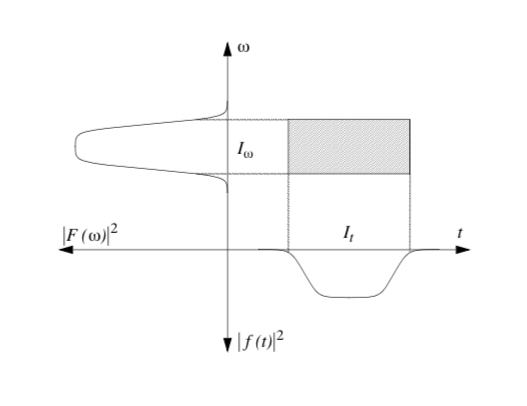
\includegraphics[width=8cm]{images/tf.png}
\caption{Representación plano tiempo-frecuencia obtenida de    \cite{waveletsandsubbandcoding}}
\end{figure}




\subsection{Aproximaciones multiresolución}

Cuando se quiere analizar una señal a diferentes escalas, es común dividir el factor de escala en 2 sucesivamente para tener cada vez más alta \emph{resolución}. La resolución se define como el inverso de la escala   \cite{wavelettour}. En nuestro estudio de wavelets es deseable encontrar wavelets que sean bases ortogonales para $L_2(\mathds{R})$. La aproximación de una función $f$ a una resolución $2^{-j}$ se define como una proyección ortogonal en un espacio $\mathcal{V}_j \subset L_2(\mathds{R})$, donde el espacio $\mathcal{V}_j$ contiene todas las aproximaciones posibles con resolución $2^{-j}$. La aproximación de $f$ en $\mathcal{V}_j$ corresponde a $f_j \in \mathcal{V}_j$ tal que el error $||f-f_j||$ sea minimizado    \cite{wavelettour, waveletsandsubbandcoding}.

\subsection{Downsampling y Upsampling}

Para obtener la DWT con distintas representaciones en distintas resoluciones de una señal, es necesario hacer un \emph{downsampling} de la señal, esto es, reducir el número de muestras, y por ende de información, en una señal (en su conjunto la DWT no supone pérdidas de información, pero sí cada canal por separado). Por su puesto, este proceso tiene que hacerse de tal manera de no violar el teorema del muestreo, es por esto que antes de bajar la resolución de muestreo, es necesario pasar la señal por un filtro pasa bajo que se deshaga de cualquier frecuencia que puede haber sido introducida en el proceso de downsampling    \cite{dwt}. De manera similar, para computar la transformada inversa IDWT, es necesario hacer \emph{upsampling} de las señales antes pasadas por el proceso de downsampling. De igual manera que en el proceso de downsampling, las señales deben pasarse por filtros para evitar la introducción de frecuencias originalmente no presentes en la señal.

\subsubsection{Decimation}

Dada una señal $x[n]$, la versión de esa señal luego de pasar por un proceso de downsampling a un factor de $M$, con $M \in \mathds{N}^*$, viene dada por:

\begin{equation}
  x_d[n] = x[Mn]
\end{equation}

Asumiendo que la señal $x[n]$ está muestreada de manera correcta\footnote{siguiendo el teorema del muestreo}, la señal se compone de frecuencias hasta $f_s/2$ donde $f_s$ es la frecuencia de muestreo de la señal. Al bajar el número de muestras, la frecuencia de muestreo pasa de ser $f_s$ a $f_s/M$. Esto quiere decir que solo los componentes con frecuencia hasta $f_s/(2M)$ pueden ser representados sin ambigüedad.

Para prevenir aliasing en la versión $x_d[n]$, la señal original primero se pasa por un filtro pasa-bajo con frecuencia de corte $f_s/(2M)$ se ejecuta la acción de downsampling.

Por su puesto es deseable evitar hacer ambas operaciones (filtrado y downsampling) de manera secuencial. Afortunadamente, ambas operaciones pueden ser hechas a la vez.

Dado un filtro $h[n]$, efectuar ambas operaciones a la vez corresponde a:

\begin{equation}
  y[n] = \sum_k h[k]x[2n-k] = \sum_k x[k]h[2n-k]
\end{equation}

Este proceso es llamado \emph{decimation} y es fundamental en el cálculo de la DWT    \cite{dwt}.



\subsubsection{Interpolación}

El proceso inverso a \emph{decimation} es la \emph{interpolación}, que consiste en \emph{upsampling} seguido de un filtro pasa bajo   \cite{dwt}.

El upsampling de una señal $x[n]$ en un factor de M se define como:

\begin{equation}
  x_u[n] =
  \begin{cases}
    x\left[\frac{n}{M}\right], \quad n = iM, i \in \mathcal{Z}\\
    0 \quad \text{en otro caso}
  \end{cases}
\end{equation}


Evidentemente, al igual que en el caso anterior, cambiar la tasa de muestreo de una señal afecta las frecuencias presentes en la misma. Es por esto que seguido del upsampling es necesario filtrar estos nuevos componentes que se pueden haber generado.

En este proceso tenemos que al hacer el upsampling, aproximadamente la mitad de los valores son iguales a 0. Por lo mismo es que es una pérdida de recursos computacionales calcular esto si ya sabemos de antemano el resultado. Es posible intercambiar el filtrado con el upsampling si el filtro $h[n]$ es pasado por un upsampling primero (usaremos $M=2$ ya que es lo común)

\begin{equation}
  h_u[n] = \{h[0], 0, h[1], 0, h[2], \hdots, h[N-1]\}
\end{equation}

Es más eficiente hacer el downsampling luego de usar el filtro ya que nos ahorra tiempo en calcular multiplicaciones con coeficientes iguales a 0.


\subsection{Wavelet Haar}

Existen infinitas wavelets   \cite{wavelettour}, pero de todas ellas, en este trabajo vamos a usar la wavelet Haar por su simplicidad.

La wavelet Haar se define de la siguiente manera:

\begin{equation}
  \Psi(t) = \begin{cases}
    -1 &\text{si}\quad 0\leq t<1/2\\
    1 &\text{si}\quad 1/2\leq t<1\\
    0 &\text{en otro caso}
\end{cases}
\end{equation}

y su función de escala es


\begin{equation}
  \Phi = \pmb{1}_{[0,1]}
\end{equation}

Esta wavelet es ortogonal \cite{wavelettour} y dentro de estas, es la wavelet con el soporte más pequeño. Además no es muy útil para aproximar funciones suaves ya que solo tiene un momento que se cancela, y la cantidad de momentos cancelados tiene directa relación con el tipo de funciones para las cuales una wavelet es más útil \cite{wavelettour}

El hecho que la wavelet Haar posee solo un momento nulo no es difícil de demostrar, por lo que a continuación lo haremos. El n-ésimo momento viene dado por
\begin{equation}
    \begin{aligned}
            \int_{-\infty}^\infty t^n \Psi(t)dt &= \int_0^{1/2}t^n dt + \int_{1/2}^1 t^n dt\\
         &=\frac{1-2(1/2)^{n+1}}{n+1}
    \end{aligned}
\end{equation}


Vemos que para que esto se cumpla, el numerador tiene que ser igual a 0

\begin{equation}
    1-2\left(\frac{1}{2}\right)^{n+1} = 0 \implies \left(\frac{1}{2}\right)^{n+1} = \frac{1}{2}
\end{equation}

Vemos que la única manera que esto se cumpla es con $n=0$ por lo que es solo ese momento el que desaparece. Que es el momento que la definición de wavelet exige, por lo que no es sorpresa que al menos ese se cumpla.



\section{Implementación de wavelet Haar en Python}

La implementación de los filtros que forman la base Haar fue hecha en Python usando recursión para generar las distintas matrices de transformación de manera eficiente. Se creó un objeto llamado \emph{HaarFilterBank} que recibe una imagen de dimensiones $N\text{x}N$ donde $N=2^J$ con $J \in \mathds{N}^*$, una vez recibida esa imagen en forma de matriz, se calculan las matrices de transformación usando las siguientes relaciones:

\begin{equation}
\pmb{W}_{N, \log_2(N)-1} =
\begin{pmatrix}
\pmb{I}_{\frac{N}{2}} \otimes \left[\frac{1}{\sqrt{2}} \qquad \frac{1}{\sqrt{2}}\right]\\
\pmb{I}_{\frac{N}{2}} \otimes \left[\frac{1}{\sqrt{2}} \quad -\frac{1}{\sqrt{2}}\right]
\end{pmatrix}
\end{equation}


\begin{equation}
\pmb{W}_{N, j} =
\begin{pmatrix}
\pmb{W}_{\frac{N}{2}, j} \otimes \left[\frac{1}{\sqrt{2}} \qquad \frac{1}{\sqrt{2}}\right]\\
\pmb{I}_{\frac{N}{2}} \otimes \left[\frac{1}{\sqrt{2}} \quad -\frac{1}{\sqrt{2}}\right]
\end{pmatrix}, \qquad j=0,1,...,\log_2(N)-2
\end{equation}


Donde $N$ es el tamaño de la matriz cuadrada y $\pmb{I}_N$ es la identidad de tamaño $N$. Para una matriz $\pmb{A}$ de $M\text{x}N$ y $\pmb{B}$ una matriz de $P\text{x}Q$, $\otimes$ representa el \emph{producto de Kronecker} definido como:

\begin{equation}
\pmb{A} \otimes \pmb{B} = a_{i, j}\pmb{B} =
\begin{pmatrix}
a_{1,1}\pmb{B} & a_{1,2}\pmb{B} & \cdots & a_{1,n}\pmb{B} \\
a_{2,1}\pmb{B} & a_{2,2}\pmb{B} & \cdots & a_{2,n}\pmb{B} \\
\vdots  & \vdots  & \ddots & \vdots  \\
a_{m,1}\pmb{B} & a_{m,2}\pmb{B} & \cdots & a_{m,n}\pmb{B}
\end{pmatrix}
\end{equation}




Dadas las relaciones anteriores, es fácil ver que la construcción de las matrices de transformación se puede implementar de manera recursiva. Además el hecho de usar el producto de Kronecker, nos muestra inmediatamente que el filtrado se está haciendo en conjunto con el downsampling, tal como habíamos explorado anteriormente.

Ahora bien, estas matrices son solo para la transformación en una dimensión, y si queremos tener las transformadas de imágenes, necesitamos extender la implementación a dos dimensiones. Para nuestra suerte, la wavelet Haar es separable, esto quiere decir que podemos hacer la transformada de las filas y luego de las columnas de la matriz que representa la imagen.


\begin{equation}
  \pmb{X} = \pmb{W}\pmb{x}\pmb{W}^T
\end{equation}

Esta relación es válida para cualquier matriz de transformación Haar de cualquier nivel, donde $\pmb{x}$ es nuestra imagen de $N\text{x}N$, $\pmb{W}$ es nuestra matriz de transformación y $\pmb{W}^T$ es la transpuesta de nuestra matriz de transformación, que también es la inversa en el caso Haar, pero al ser aplicada por el otro lado de $\pmb{x}$ equivale a tomar la transformada en el otro eje. Toda esta expresión en su conjunto generan la matriz $\pmb{X}$ que es la DWT \emph{(Discrete Wavelet Transform)} de $\pmb{x}$.





\subsection{Estructura de la Haar DWT} \label{estruct}


Una característica importante del proceso descrito anteriormednte, es que se puede interpretar como muchos filtros pasa-bajos y pasa-altos puestos en una estructura de árbol. El patrón resultante de repetir este proceso es básicamente una representación multiresolución de la señal original. Donde gracias al downsampling mantenemos el tamaño de la señal de entrada $\pmb{x}$ en la salida $\pmb{X}$.


\begin{figure}[H]
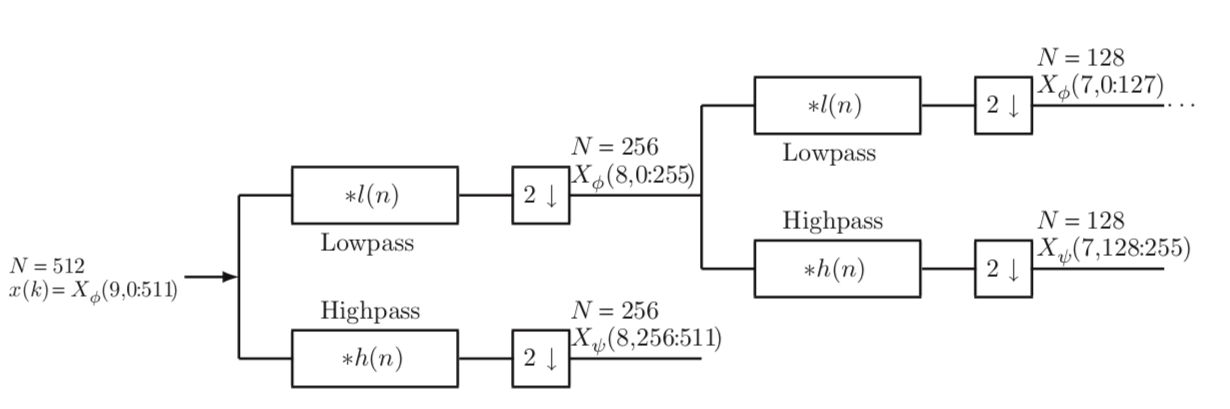
\includegraphics[width=8cm]{images/tree.png}
\caption{Estructura de árbol de la DWT. Imagen obtenida de \cite{dwt}}.
\end{figure}



En la figura notamos que hay dos notaciones para las transformadas de $\pmb{x}$, dadas por $\pmb{X}_\Phi$ y $\pmb{X}_\Psi$. Estos son los componentes de \emph{aproximación} y \emph{detalle} respectivamente. Como vimos anteriormente, son proyecciones en la wavelet con escalas grandes y escalas pequeñas. El proceso consiste en que a la parte de coeficientes de aproximación se le trata como una nueva señal y se le aplican los mismos filtros aplicados en el paso anterior y como cambiamos la escala, cambian las frecuencias de corte de manera que podemos repetir este proceso hasta lo que el tamaño de la señal lo permita. Si denotamos por $\pmb{H}$ al filtro pasa alto y $\pmb{L}$ al filtro pasa bajo. La estructura de la DWT de $\pmb{x}$ puede verse como


\begin{equation}
    \pmb{X} = \pmb{W}\pmb{x}\pmb{W}^T =
    \begin{pmatrix}
        \pmb{L}\pmb{x}\pmb{L}^T & \pmb{L}\pmb{x}\pmb{H}^T \\
        \pmb{H}\pmb{x}\pmb{L}^T & \pmb{H}\pmb{x}\pmb{H}^T
    \end{pmatrix}
\end{equation}


Vemos que equivale a aplicar filtros en las columnas seguido por filtros en las filas, y así para cada nivel. Como el proceso de downsampling está involucrado, mantenemos el mismo tamaño que la entrada $\pmb{x}$ \cite{dwt}. Este proceso puede ser iterado y lo que logramos con esto es ver todos los distintos componentes presentes en la señal para distintas escalas.

\subsection{Condiciones para la reconstrucción perfecta}

Es natural preguntarse cuáles son las condiciones para que, al transformar una señal, su inversa nos recupere la señal original de manera perfecta.

En rigor, una reconstrucción perfecta implica que los filtros de la transformada cumplen

\begin{equation}
    H(e^{j\omega})\tilde{H}(e^{j\omega}) + L(e^{j\omega})\tilde{L}(e^{j\omega}) = 1
\end{equation}

Pero como los filtros no son perfectos y siempre va a haber parte de ellos con aliasing entre sí, nos conformamos con que se cumpla lo siguiente \cite{dwt}. 


\begin{equation}
    H(e^{j\omega})\tilde{H}(e^{j\omega}) + L(e^{j\omega})\tilde{L}(e^{j\omega}) = Me^{jK\omega}
\end{equation}

Donde esto implica que esperamos una distorción tanto en fase como en amplitud. El término $H(e^{j\omega})\tilde{H}(e^{j\omega})$ es una cascada de dos sistemas con respuestas $H(e^{j\omega})$ y $\tilde{H}(e^{j\omega})$, lo mismo ocurre para el otro término en la relación anterior. La suma equivale a ponerlos en paralelo como en figura.




\begin{figure}[H]
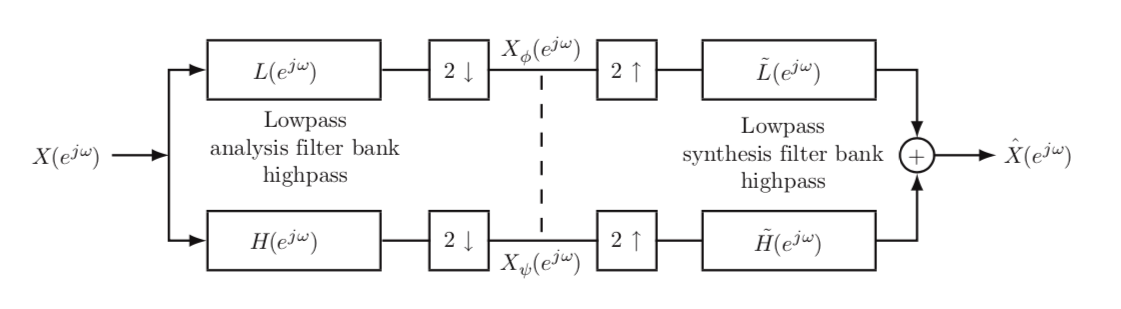
\includegraphics[width=8cm]{images/filter.png}
\caption{Representación en dominio de frecuencia de dos bancos de análisis y síntesis. Imagen obtenida de \cite{dwt}}
\end{figure}


\section{Resultados Experimentales}

Con el afán de experimentar qué efectos tiene utilizar la DWT de una imagen, se tomaron dos imágenes distintas; una de un tordo, ave que se puede encontrar en Santiago de Chile, y otra de un fragmento del libro \emph{Wavelets and Subband Codding} \cite{waveletsandsubbandcoding}, a continuación se presentan las imágenes recortadas para ser de tamaño $2048\text{x}2048$, notar que $2048 = 2^{11}$, las imágenes completas y el código para generar el análisis se puede encontrar en el repositorio de GitHub de este trabajo  \cite{repo}.


\begin{figure}[H]
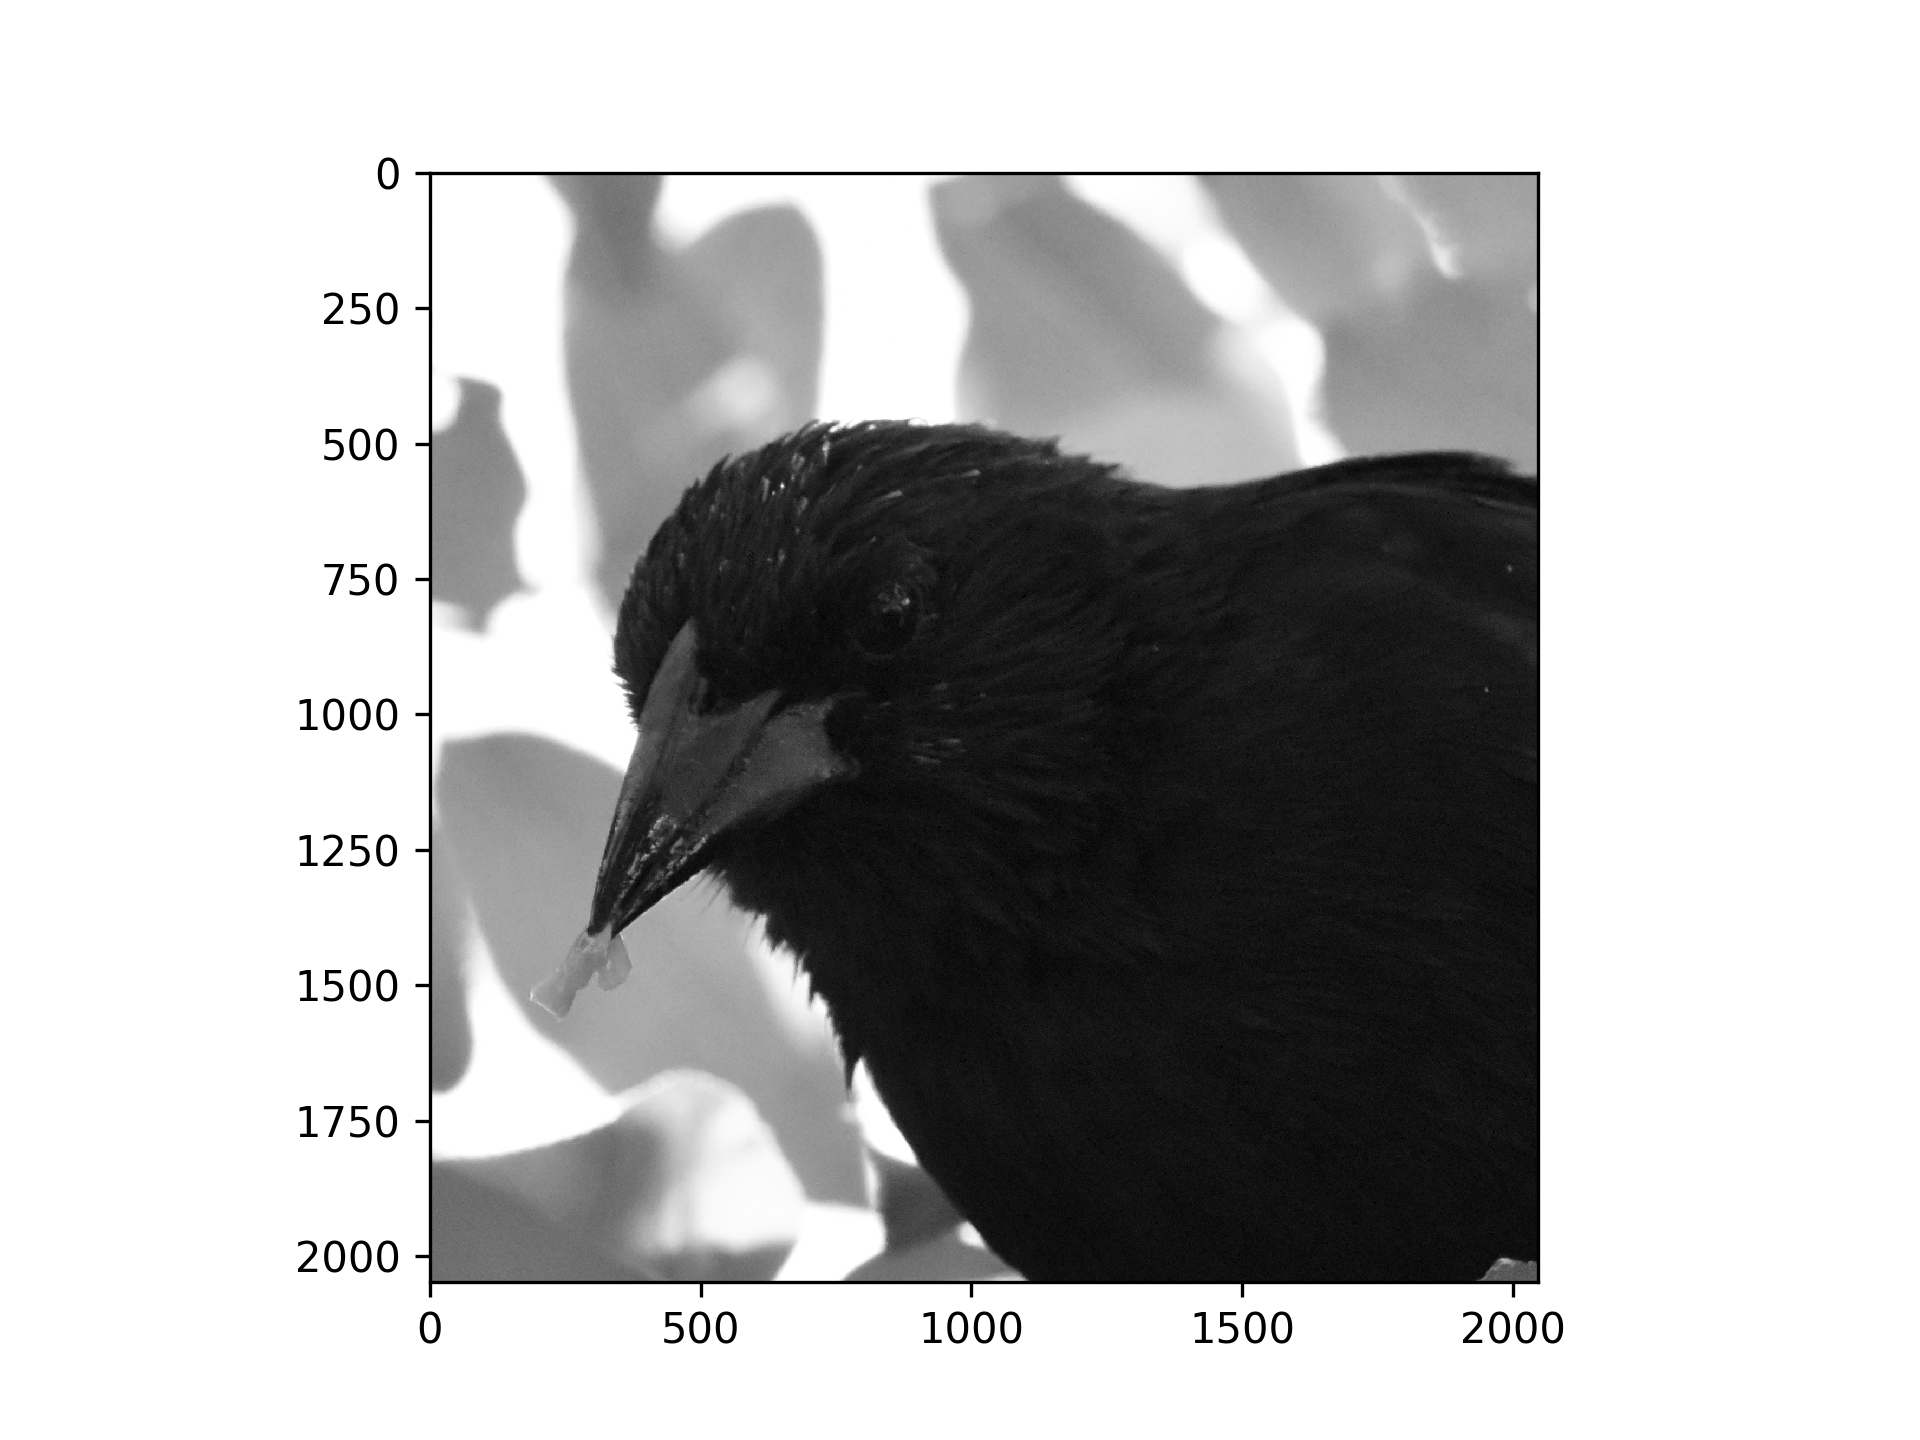
\includegraphics[width=8cm]{images/tordo_cut.png}
\caption{Tordo comiendo una ciruela amarilla. Santiago, Chile}
\end{figure}


\begin{figure}[H]
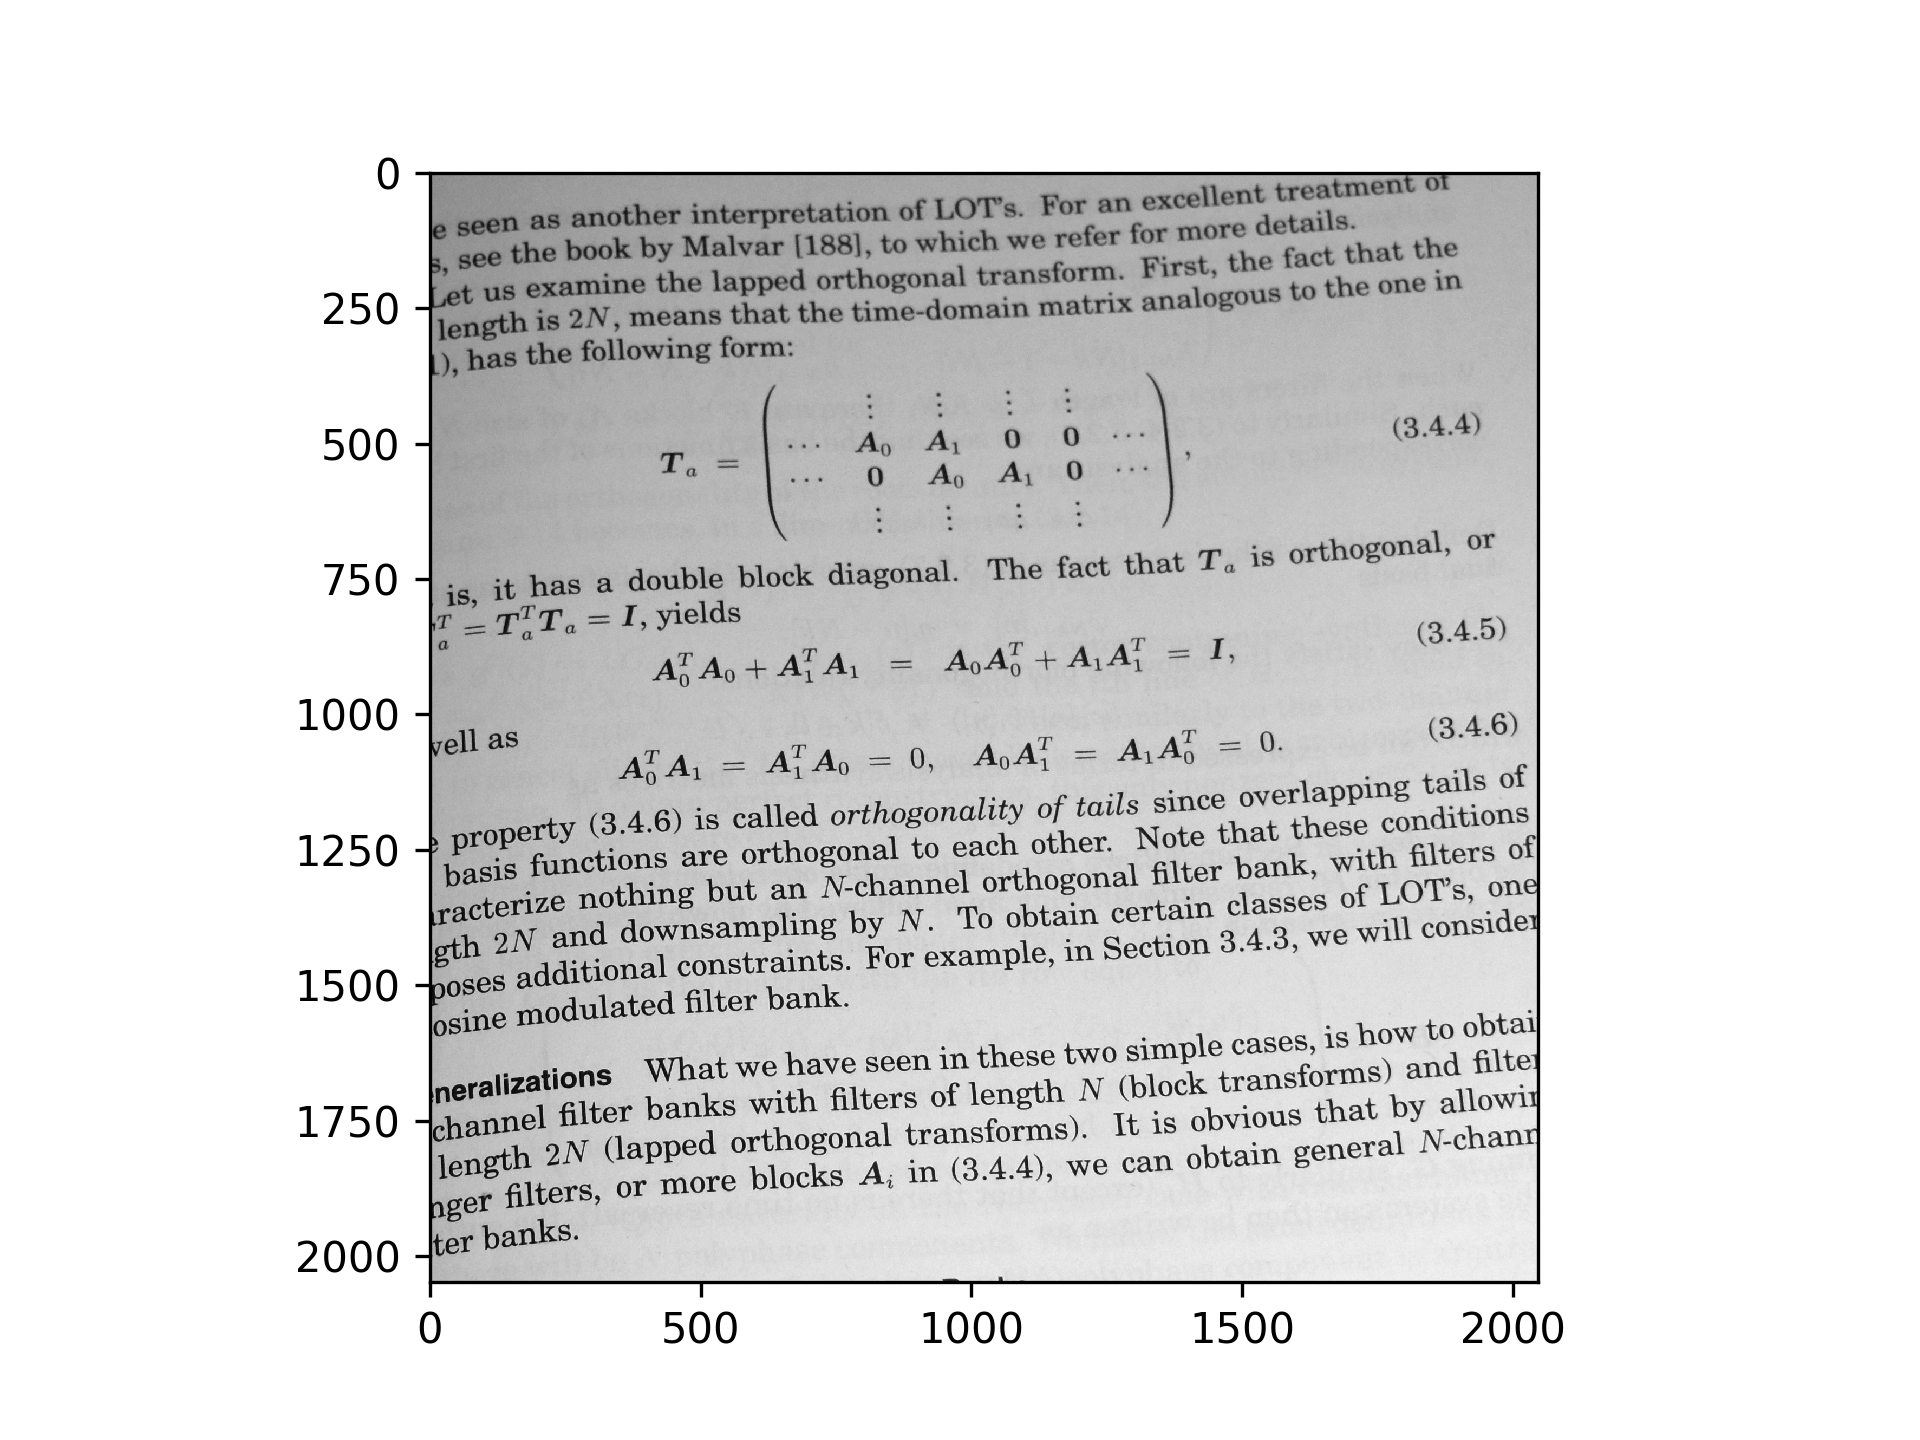
\includegraphics[width=8cm]{images/book_cut.png}
\caption{Fragmento del libro Wavelets and Subband Codding}
\end{figure}


Estas imágenes no fueron escogidas al azar. La imagen del tordo se escogió ya que en la sección recortada, no hay muchos detalles, salvo por las plumas y bordes, pero no hay detalles que sean fundamentales para comprender que es un ave. En la imagen del libro hay muchos detalles que sí son importantes para comprender de qué trata el libro. Ambas imágenes tienen características importantes a diferentes escalas (difieren de su contenido en frecuencia) y por lo tanto se espera que reaccionen de manera distinta a las wavelets.


A continuación podemos ver las DWT de ambas imágenes para el nivel 1 de análisis.

\begin{figure}[H]
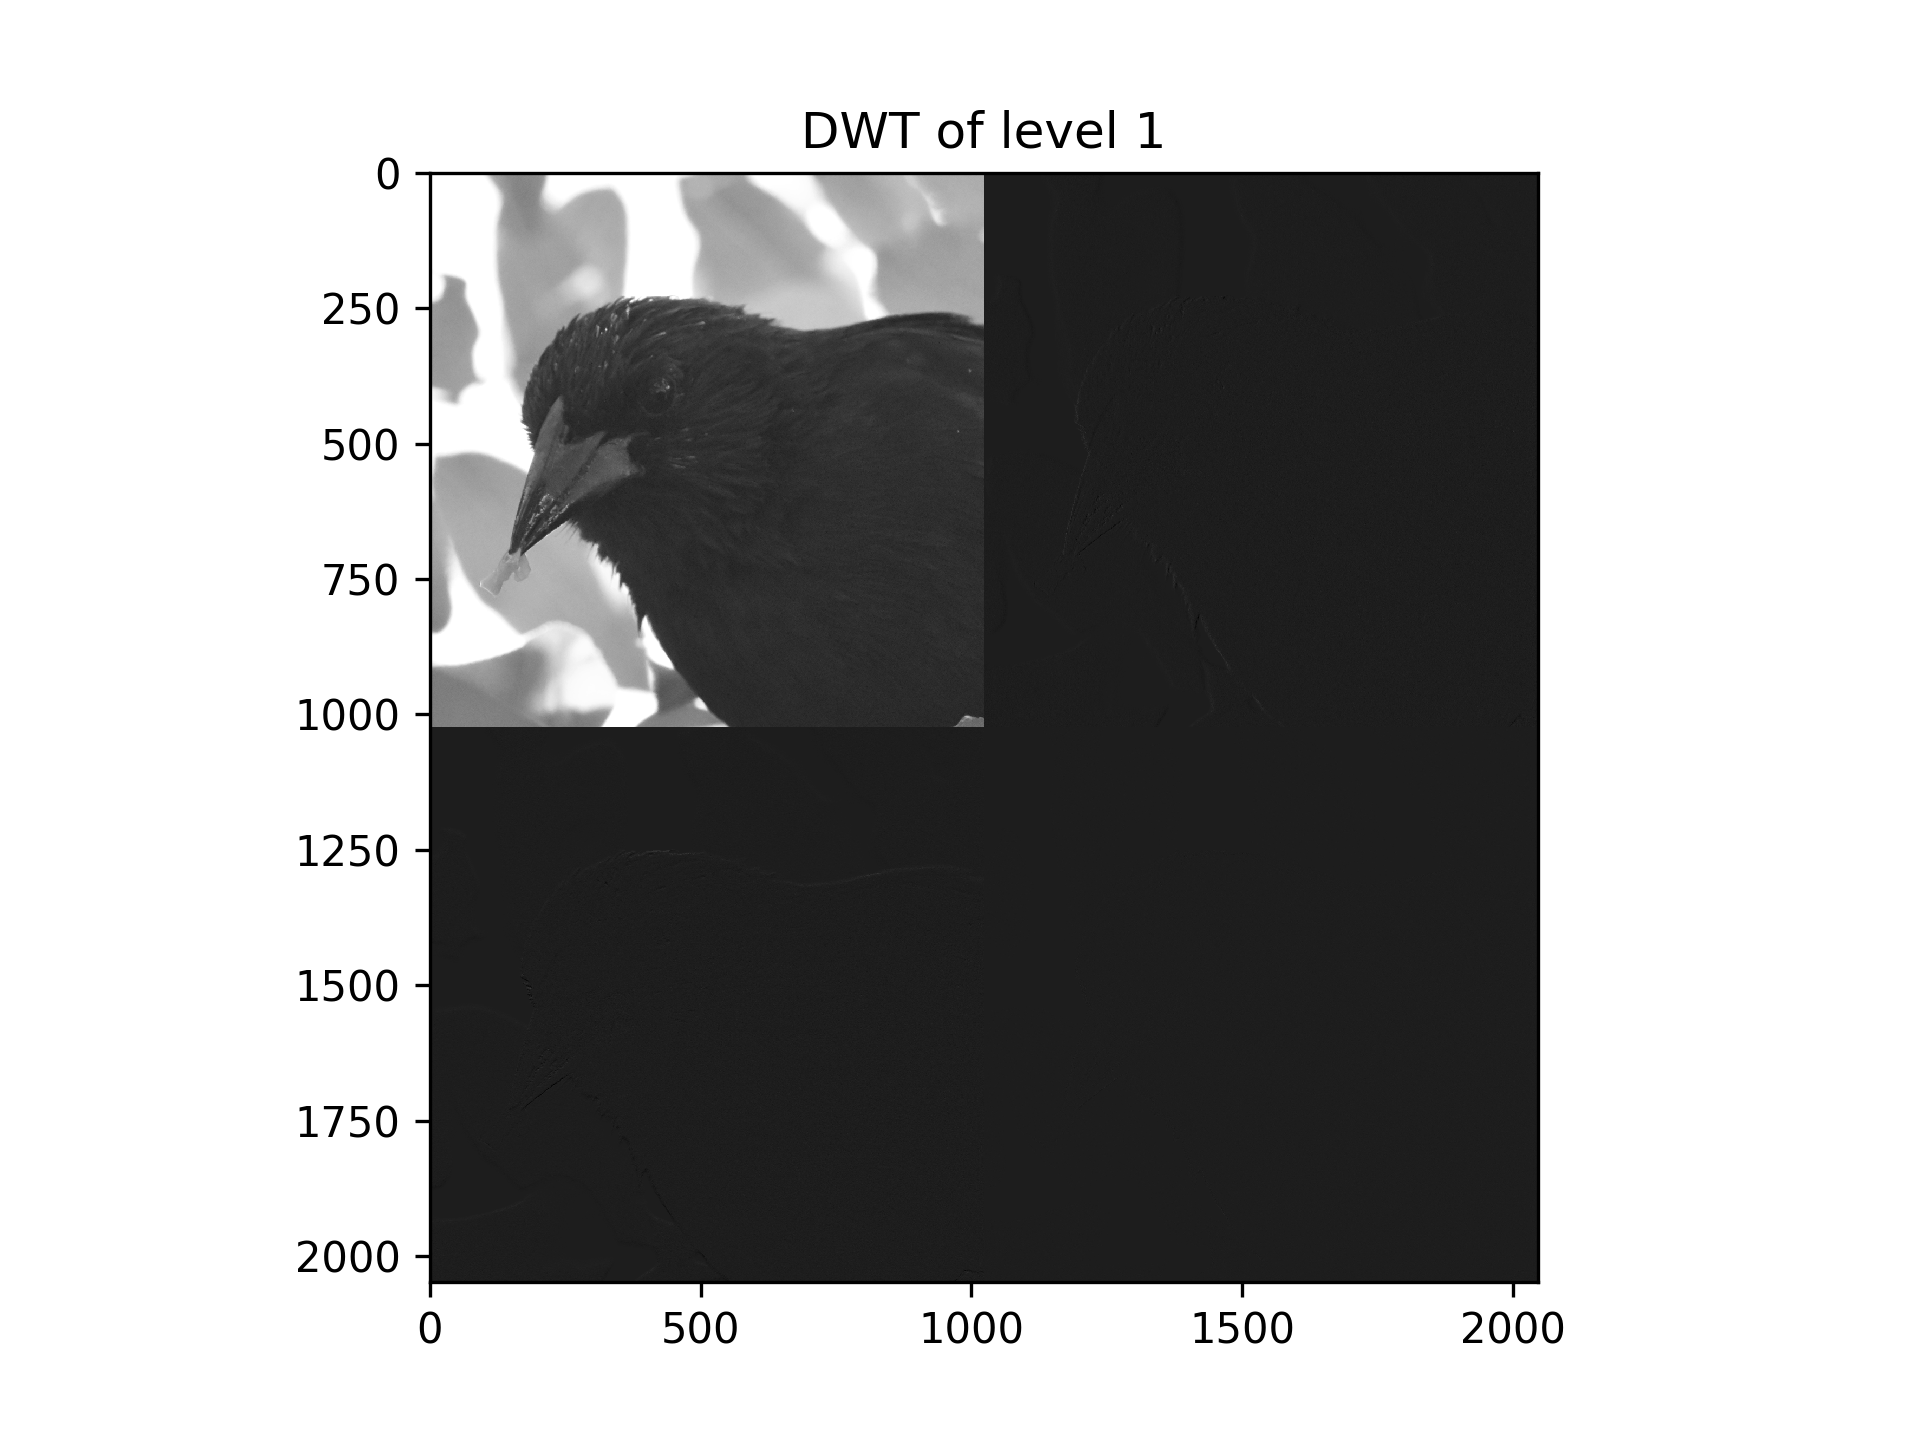
\includegraphics[width=8cm]{images/tordoDWT1.png}
\caption{DWT de nivel 1 para el tordo}
\end{figure}

\begin{figure}[H]
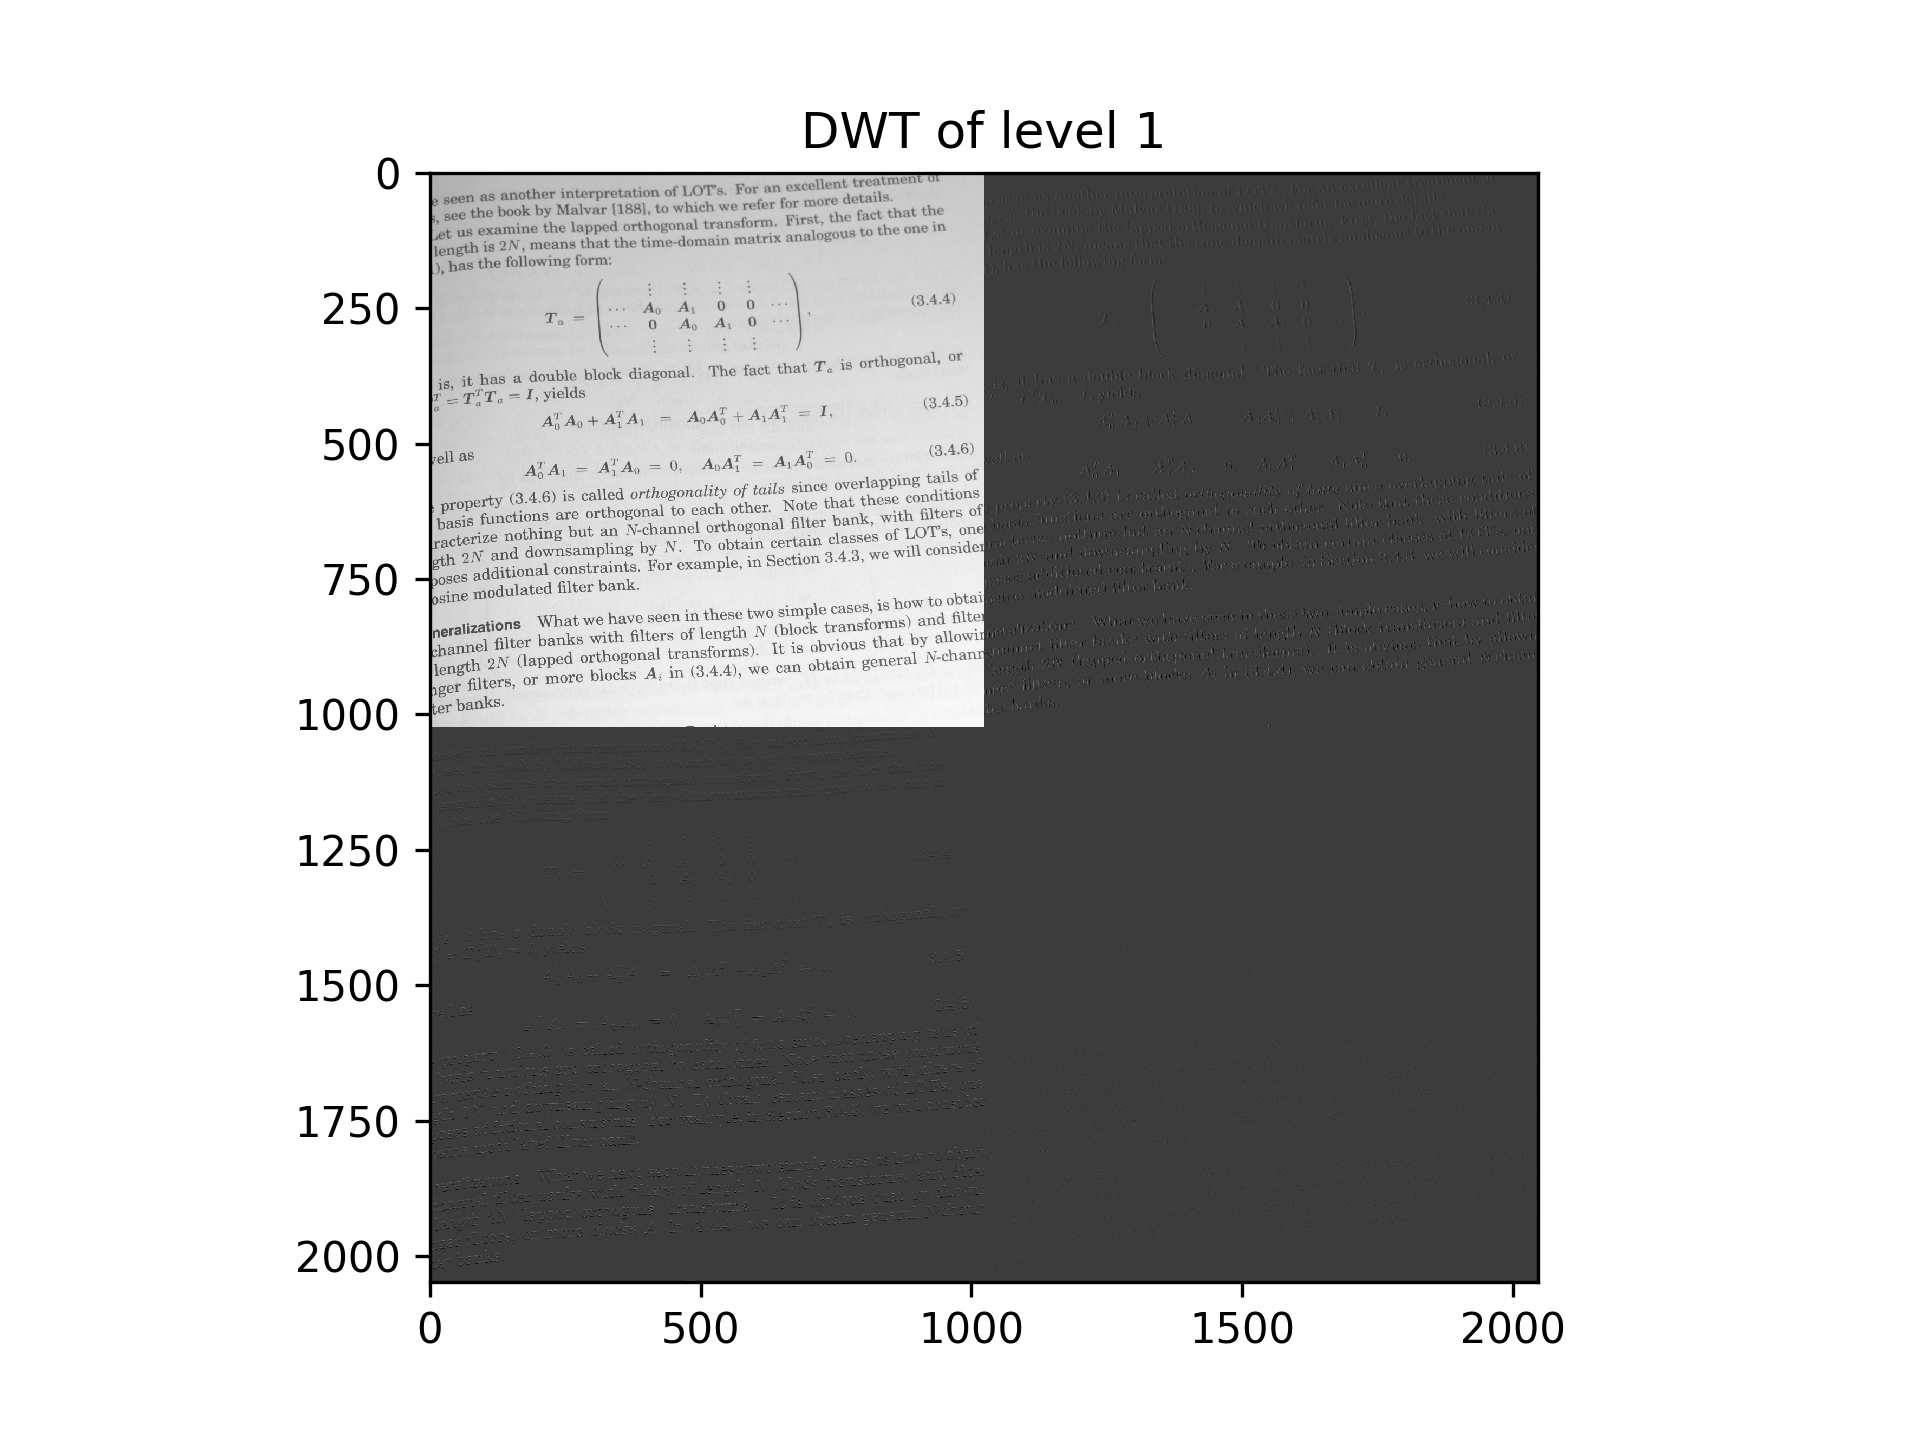
\includegraphics[width=8cm]{images/bookDWT1.png}
\caption{DWT de nivel 1 para el libro}
\end{figure}


Notar que estas transformadas siguen la estructura especificada en la sección \ref{estruct}


\subsection{Comprimiendo imágenes}

Una característica de las wavelets es que al tener soporte bien concentrado en los bajos coeficientes\cite{turbulence}, se puede comprimir una imagen sin mucho más que truncar la transformada en los coeficientes bajos y tomar la inversa para esos componentes. Acá podemos ver que incluso para la aproximación con coeficientes bajos para nivel 2 tiene una pérdida de calidad que no supone mayores problemas para fines prácticos. Los coeficientes en las siguientes dos imágenes corresponden a 1/4 y 1/8 de la información original respectivamente.


\begin{figure}[H]
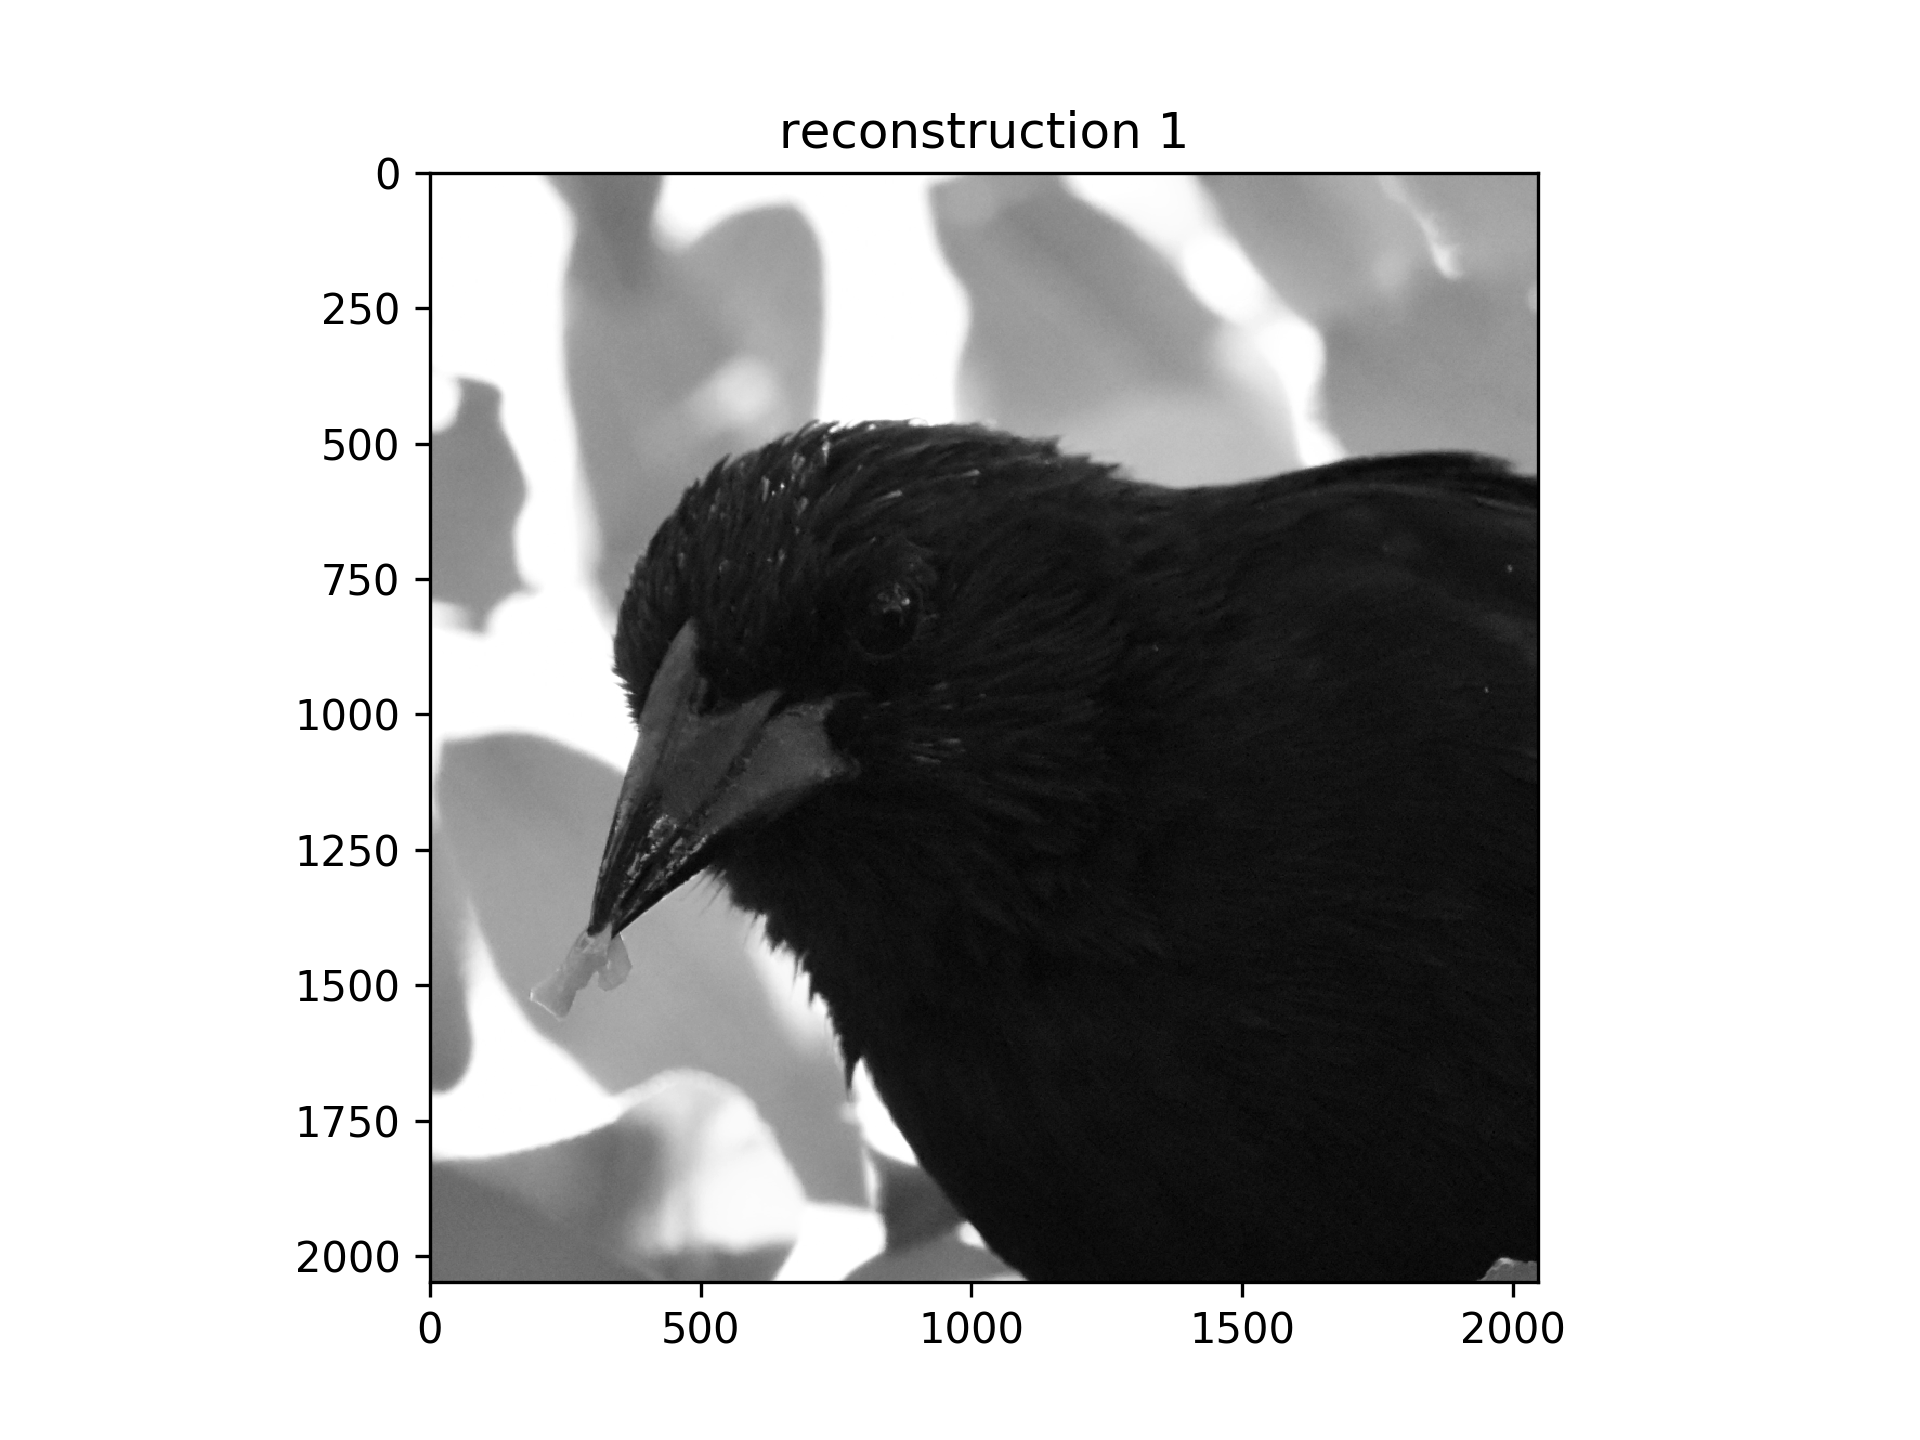
\includegraphics[width=8cm]{images/tordo_r_1.png}
\caption{Tordo reconstruido tomando 1/4 de los coeficientes de la DWT de nivel 1}
\end{figure}



\begin{figure}[H]
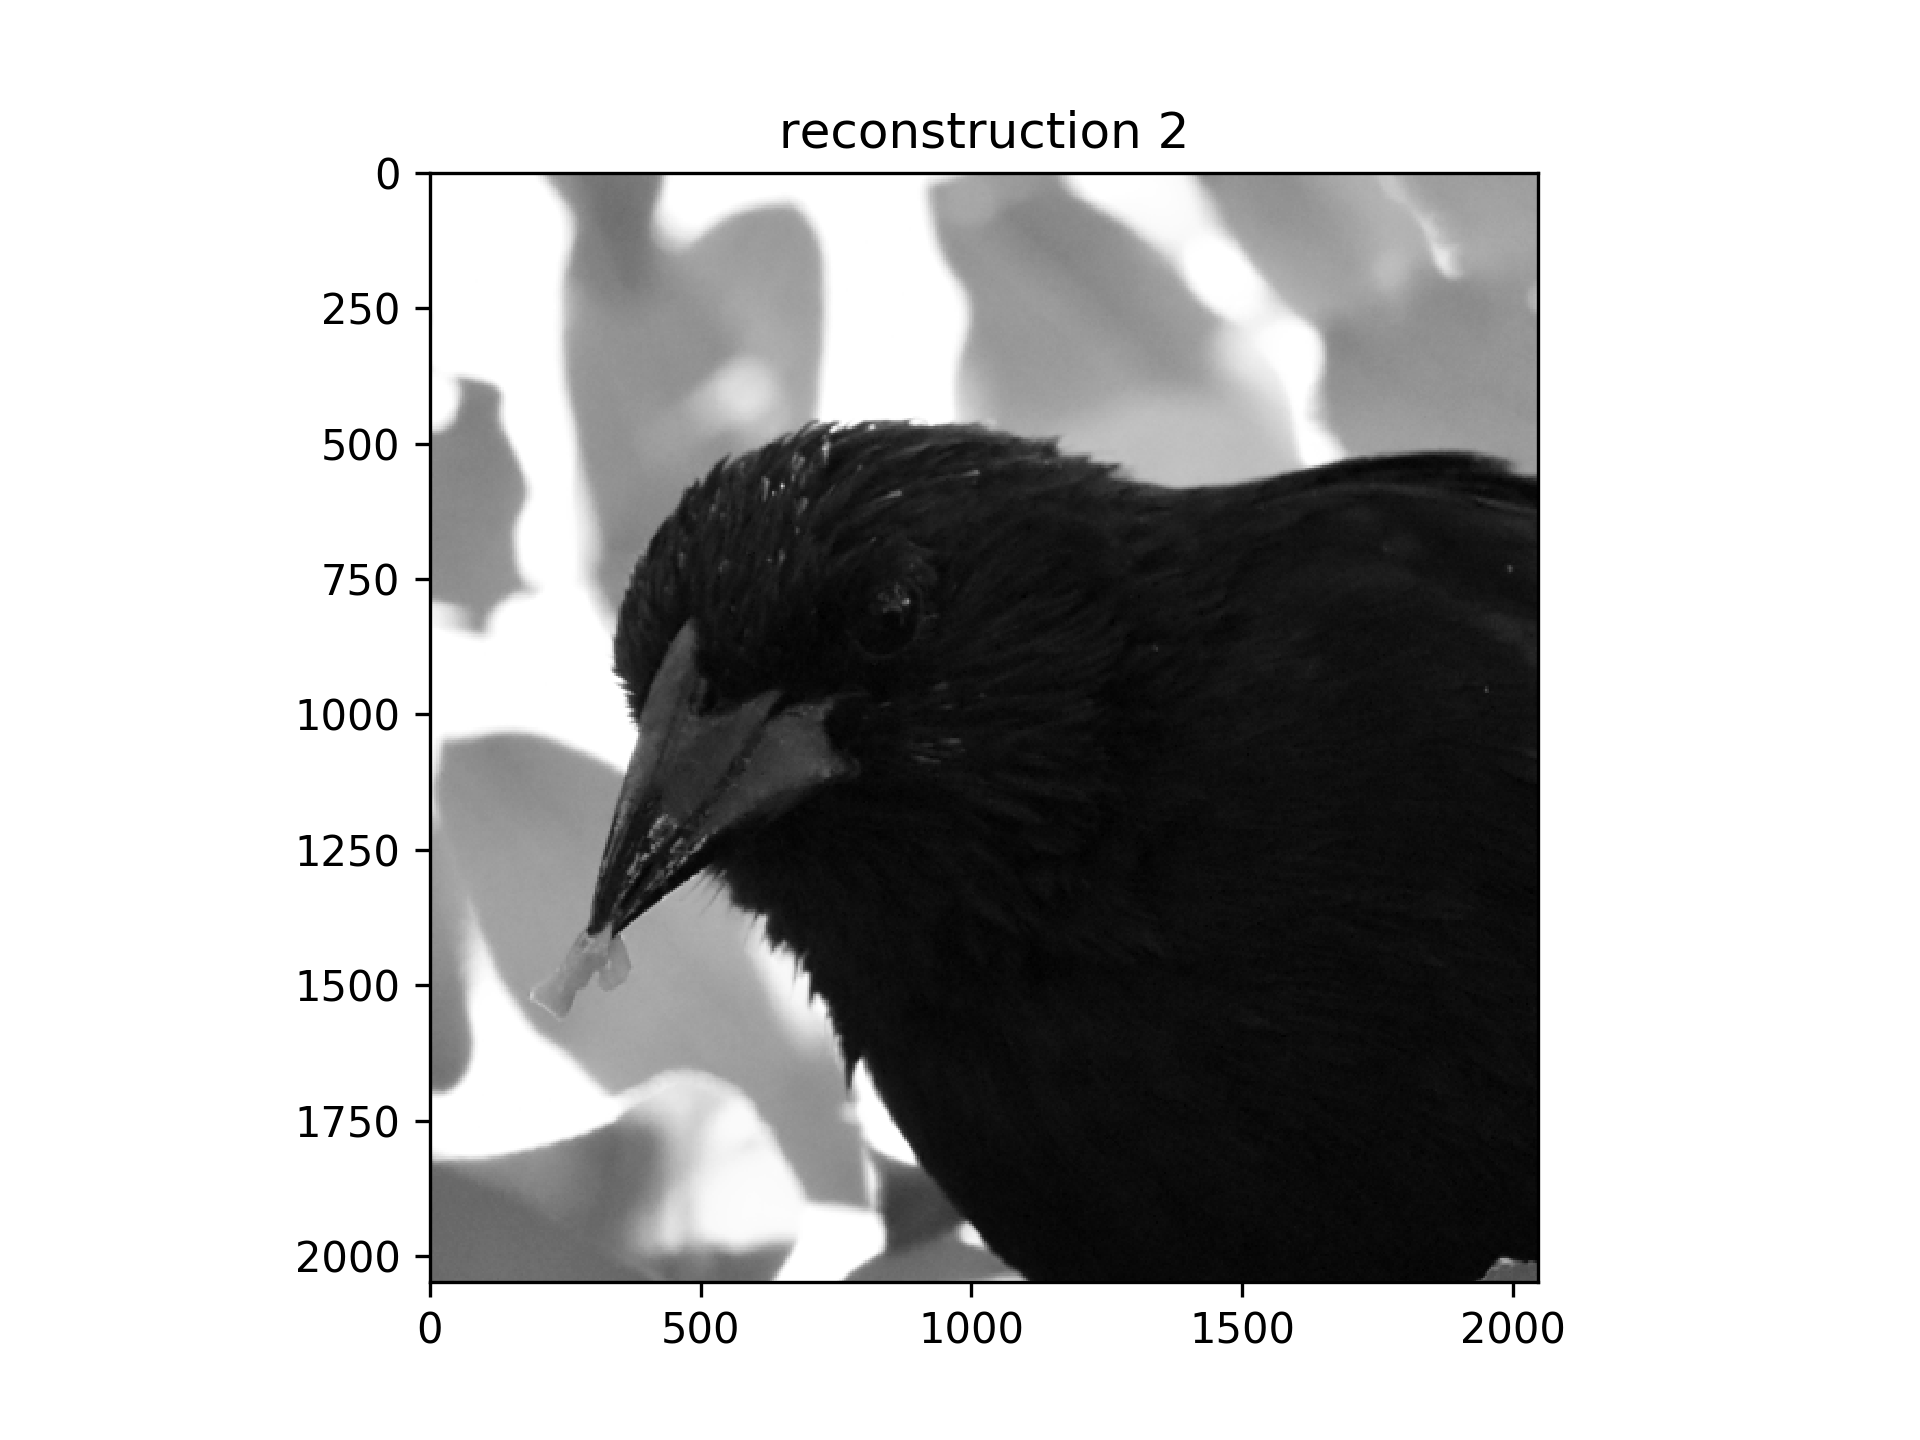
\includegraphics[width=8cm]{images/tordo_r_2.png}
\caption{Tordo reconstruido tomando 1/8 de los coeficientes de la DWT de nivel 2}
\end{figure}

\begin{figure}[H]
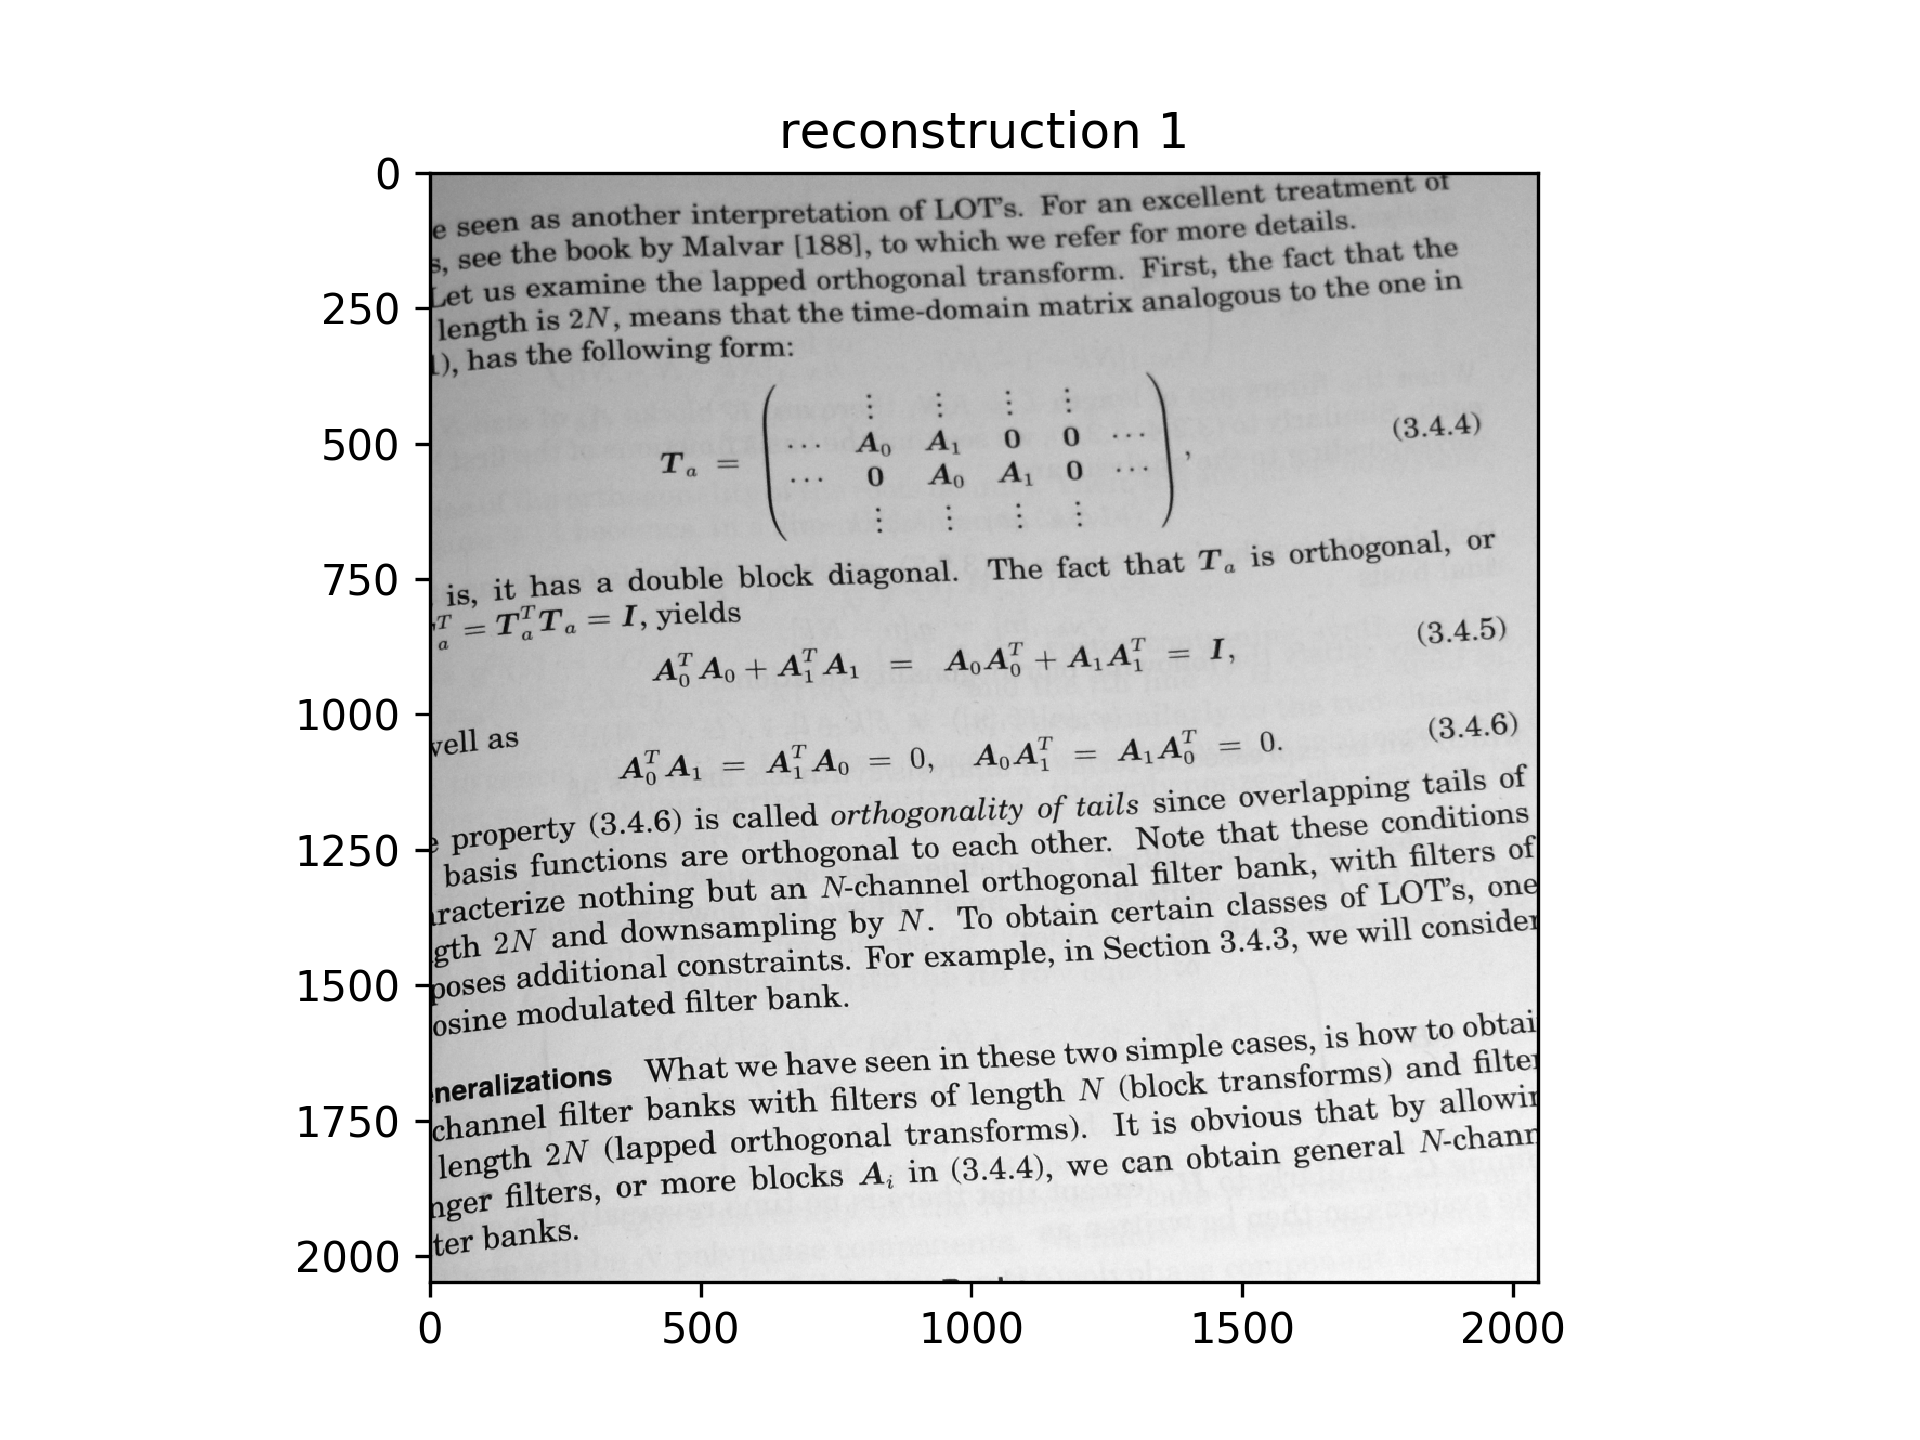
\includegraphics[width=8cm]{images/book_r_1.png}
\caption{Libro reconstruido tomando 1/4 de los coeficientes de la DWT de nivel 2}
\end{figure}

\begin{figure}[H]
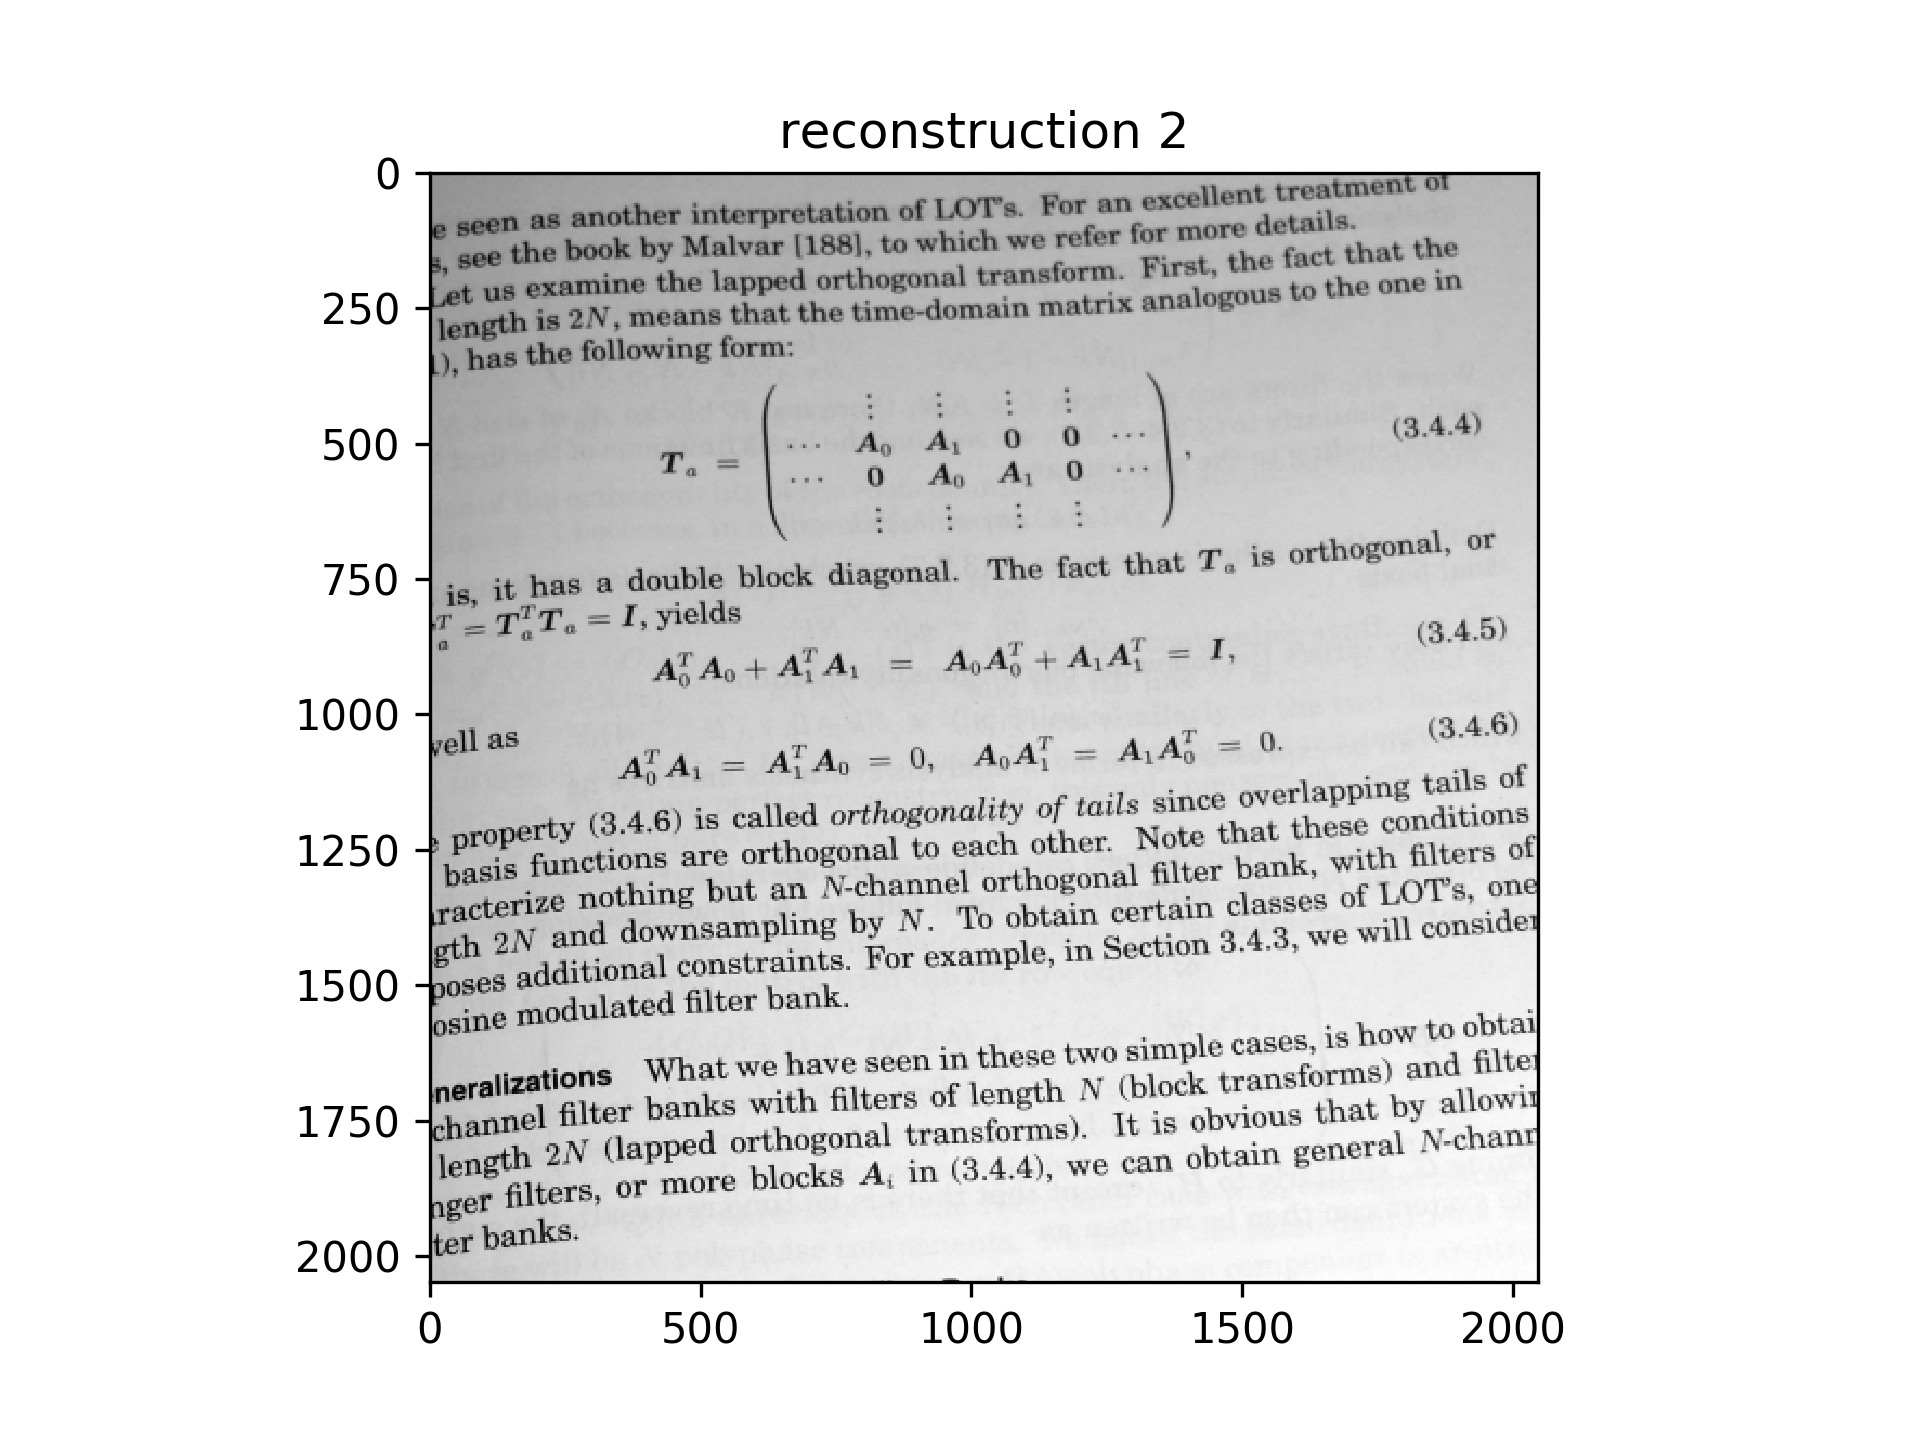
\includegraphics[width=8cm]{images/book_r_2.png}
\caption{Libro reconstruido tomando 1/8 de los coeficientes de la DWT de nivel 2}
\end{figure}

\subsection{Detección de bordes}

Como las wavelets nos ayudan a encontrar características bien localizadas, es de esperar una aplicación como la detección de bordes. Acá no vamos a implementar algoritmos de detección de bordes, solo vamos a mostrar imágenes de las cuales es fácil deducir que es una posible aplicación de las wavelets.

Hay varios algoritmos que se aprovechan de las propiedades locales de las wavelets para encontrar bordes \cite{edge1, edge2, edge3}. Para ilustrar las posibles aplicaciones, acá vemos componentes de alta frecuencia para las wavelets de nivel 5 y 6 tanto para el tordo como para el libro.

\begin{figure}[H]
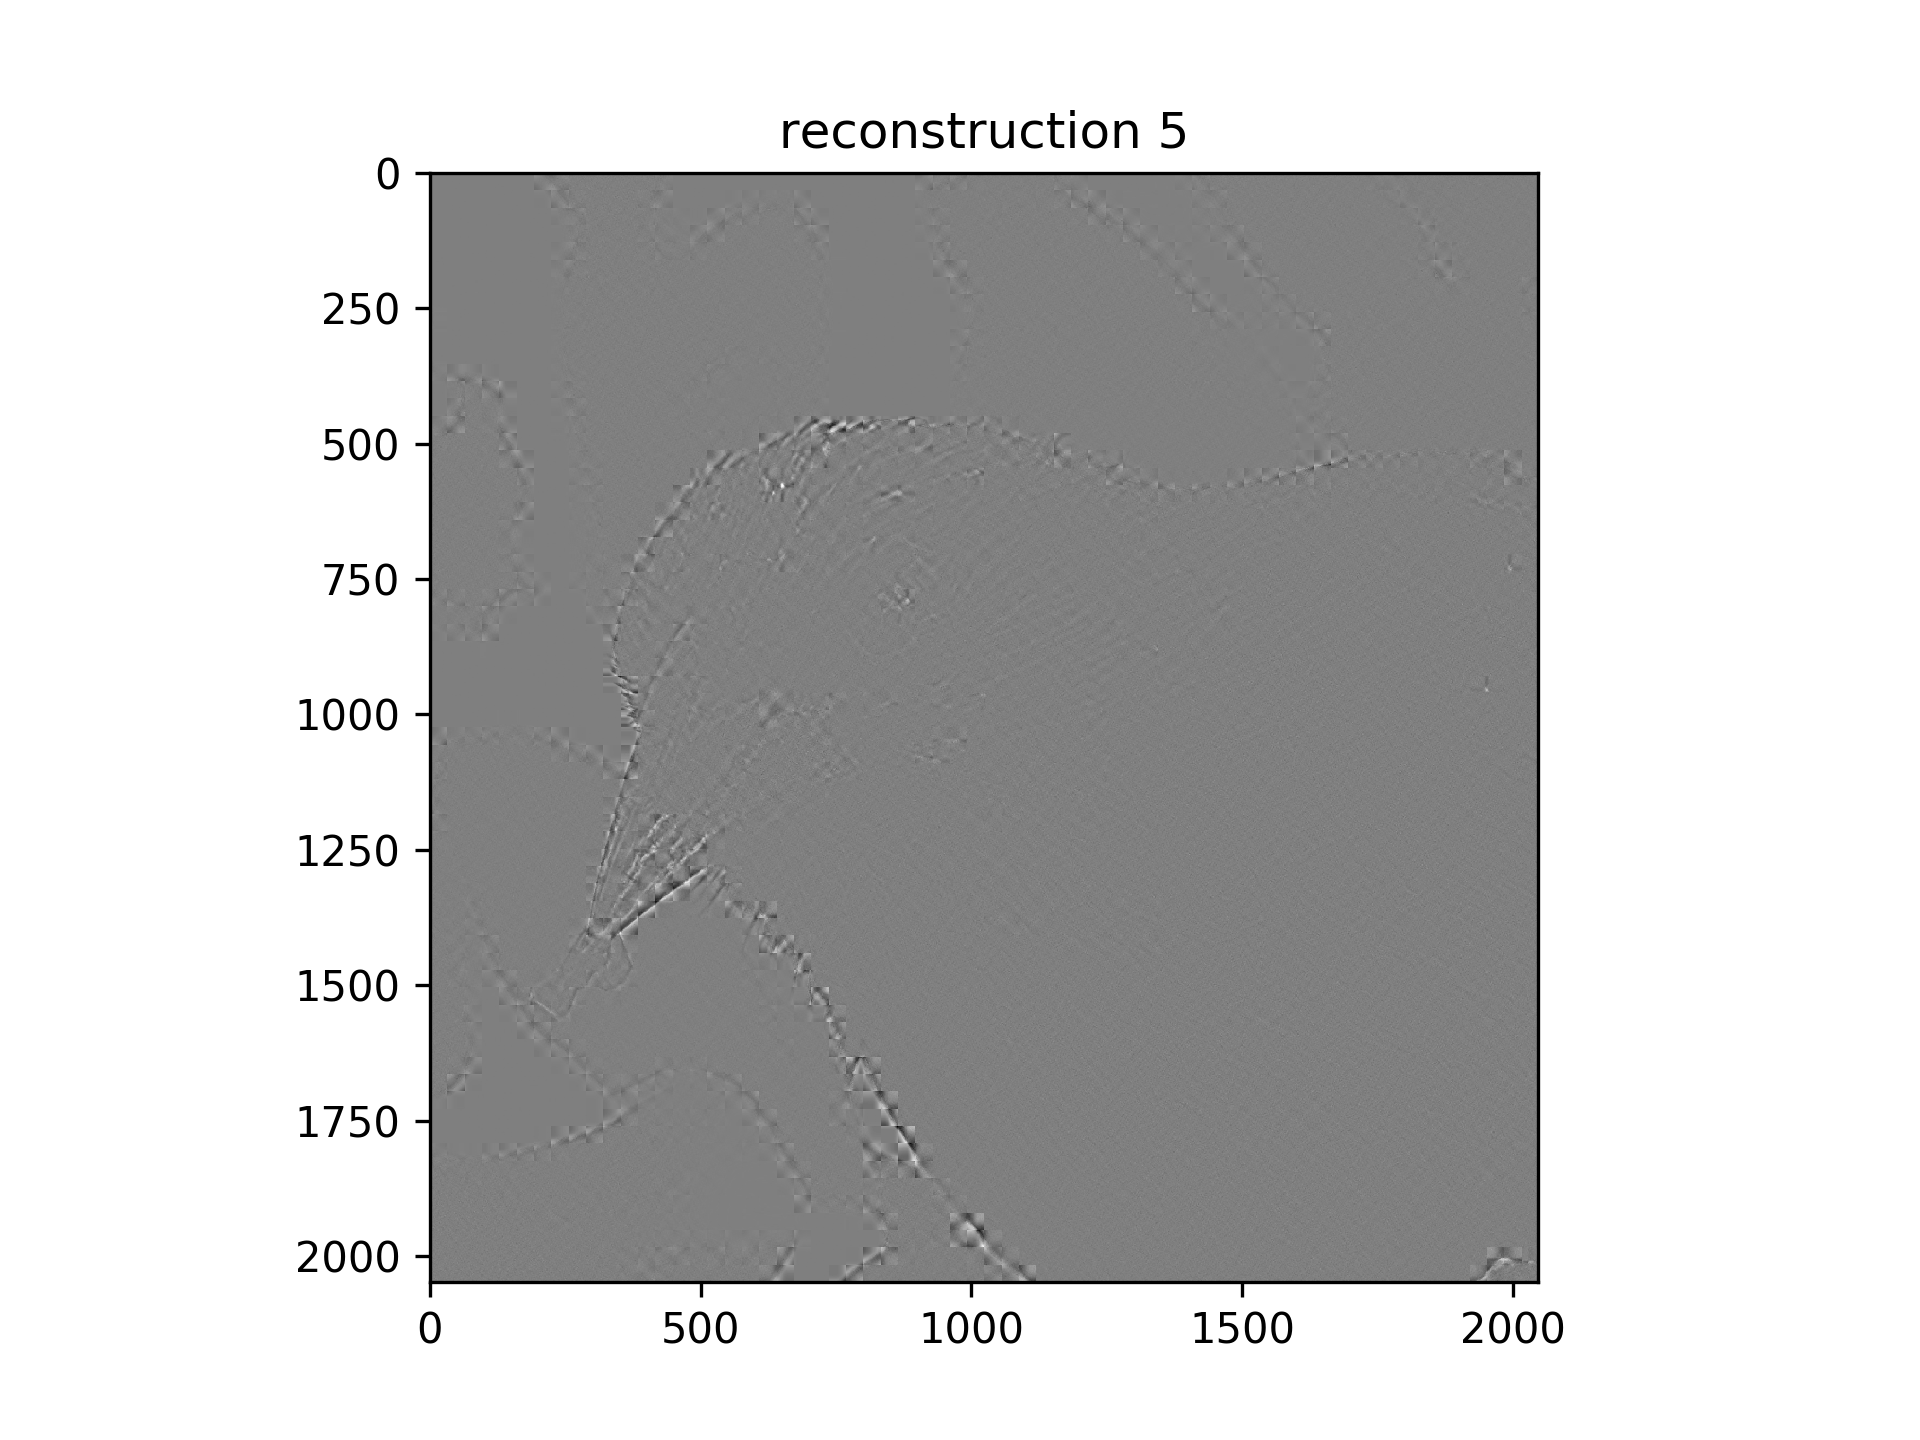
\includegraphics[width=8cm]{images/tordo_r_h_5.png}
\caption{Tordo reconstruido tomando los coeficientes más altos de la DWT de nivel 5}
\end{figure}

\begin{figure}[H]
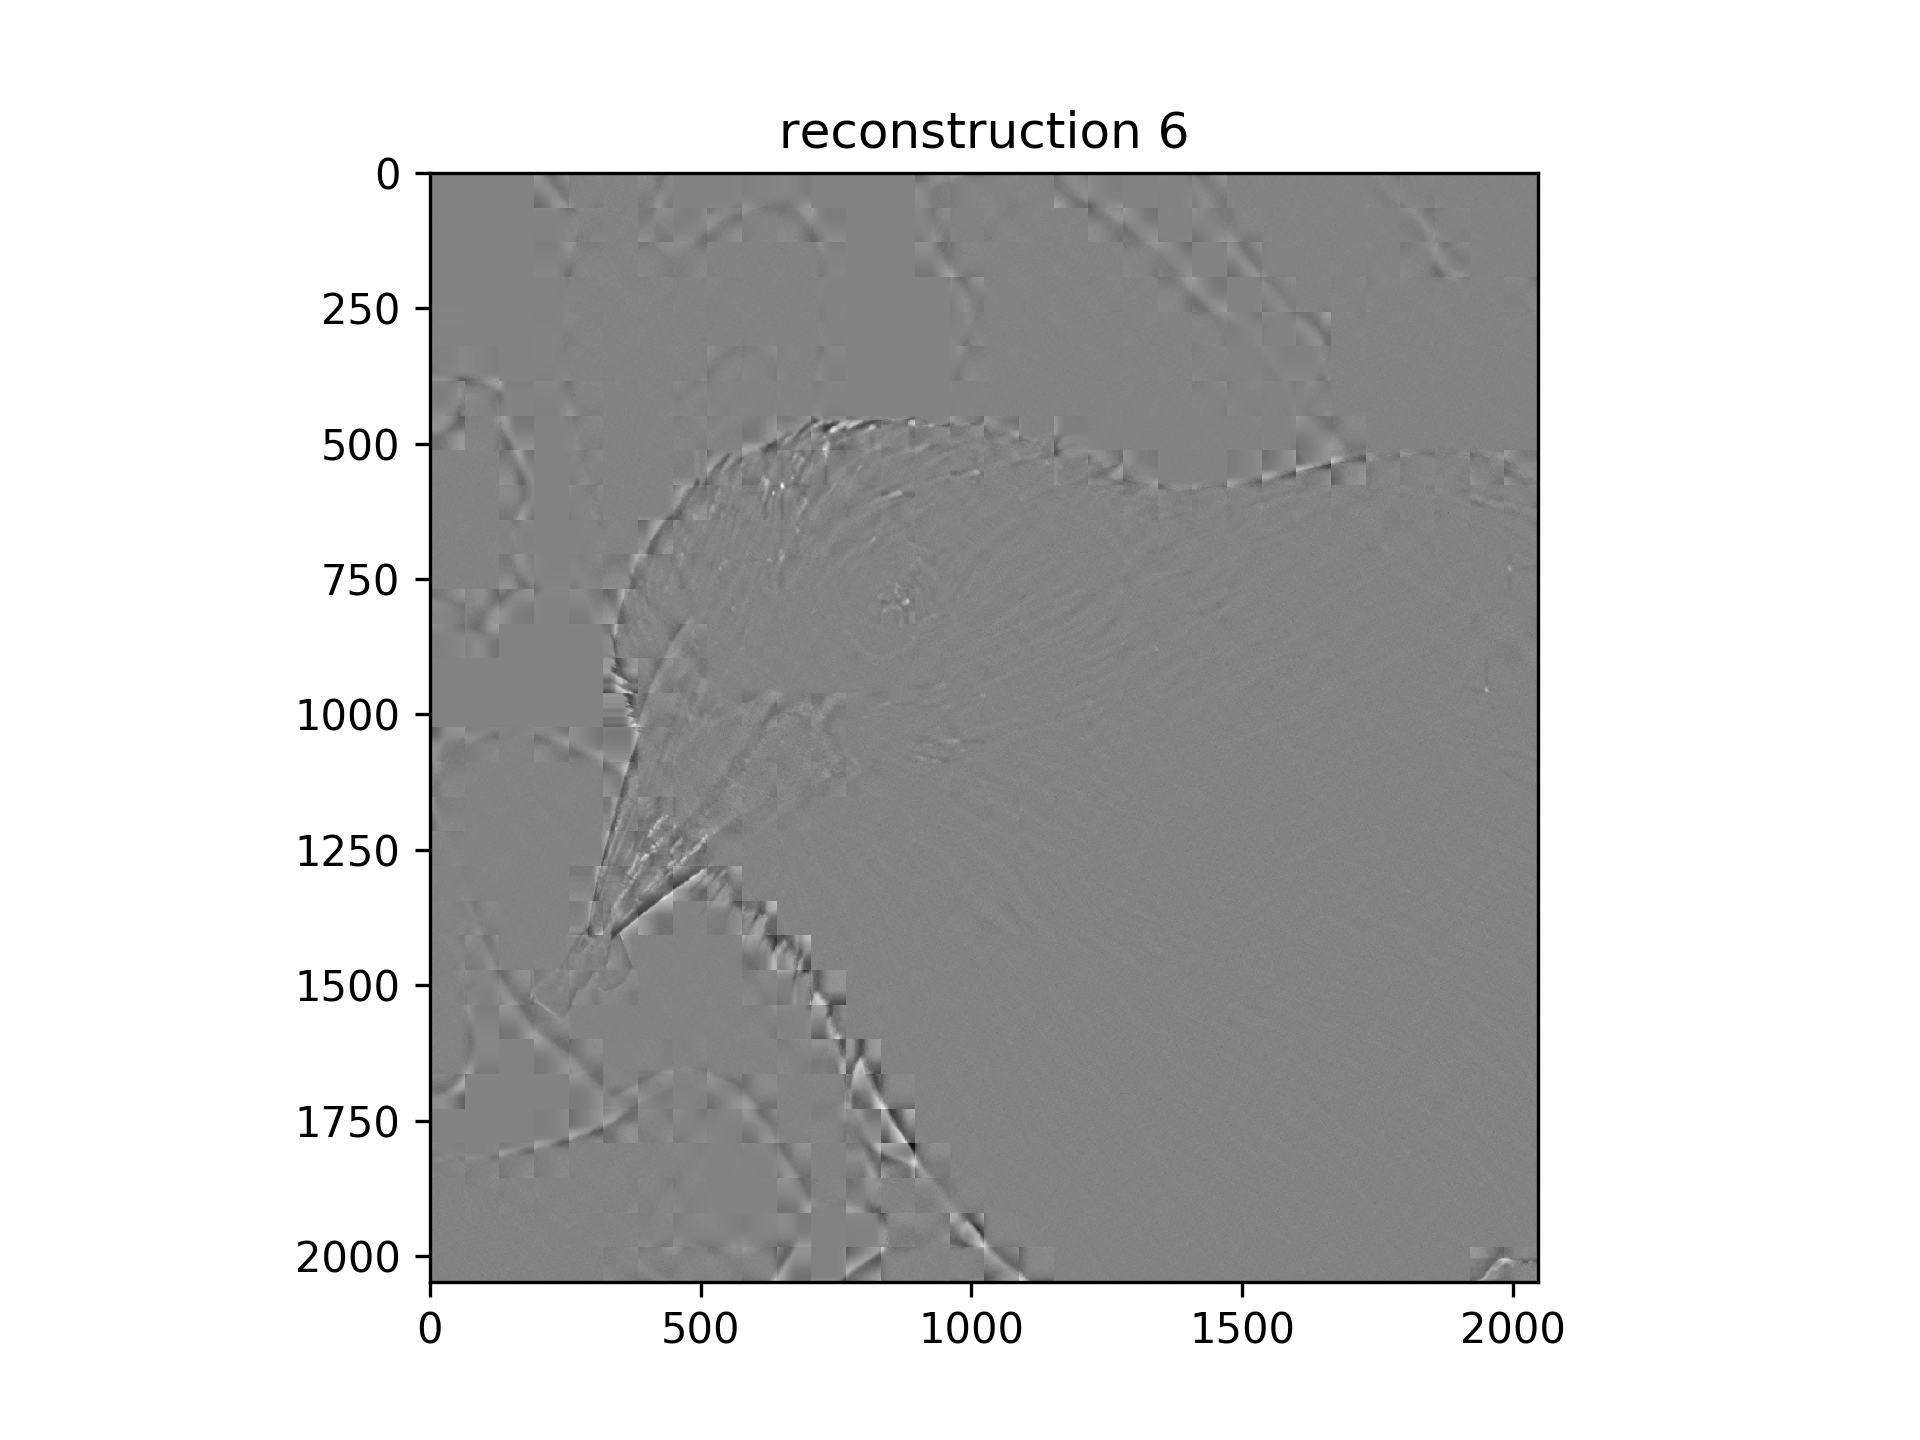
\includegraphics[width=8cm]{images/tordo_r_h_6.png}
\caption{Tordo reconstruido tomando los coeficientes más altos de la DWT de nivel 6}
\end{figure}

\begin{figure}[H]
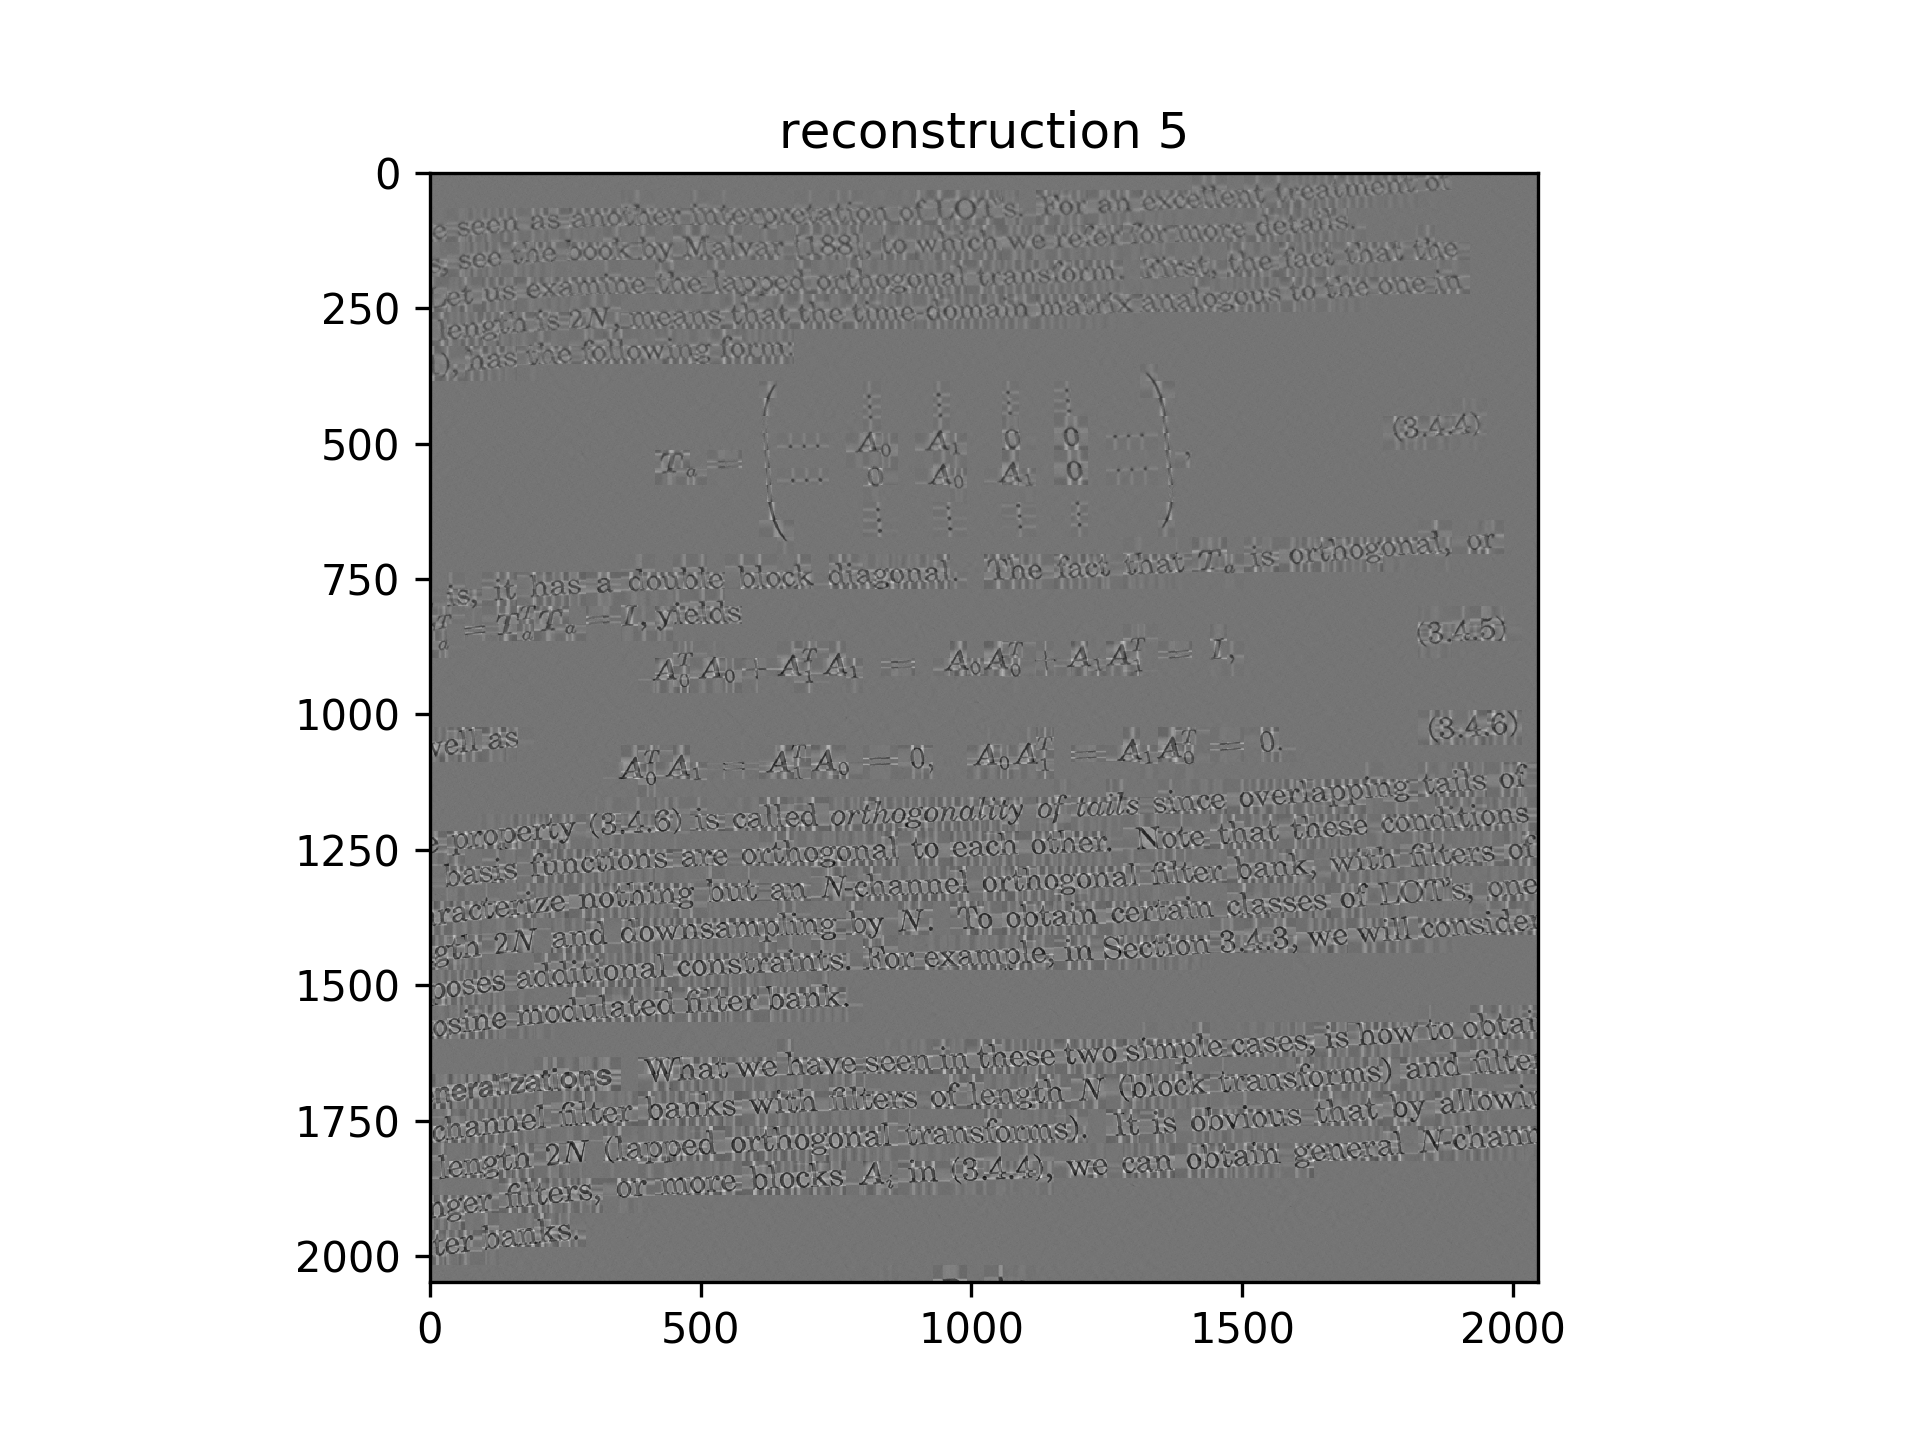
\includegraphics[width=8cm]{images/book_r_h_5.png}
\caption{Libro reconstruido tomando los coeficientes más altos de la DWT de nivel 5}
\end{figure}

\begin{figure}[H]
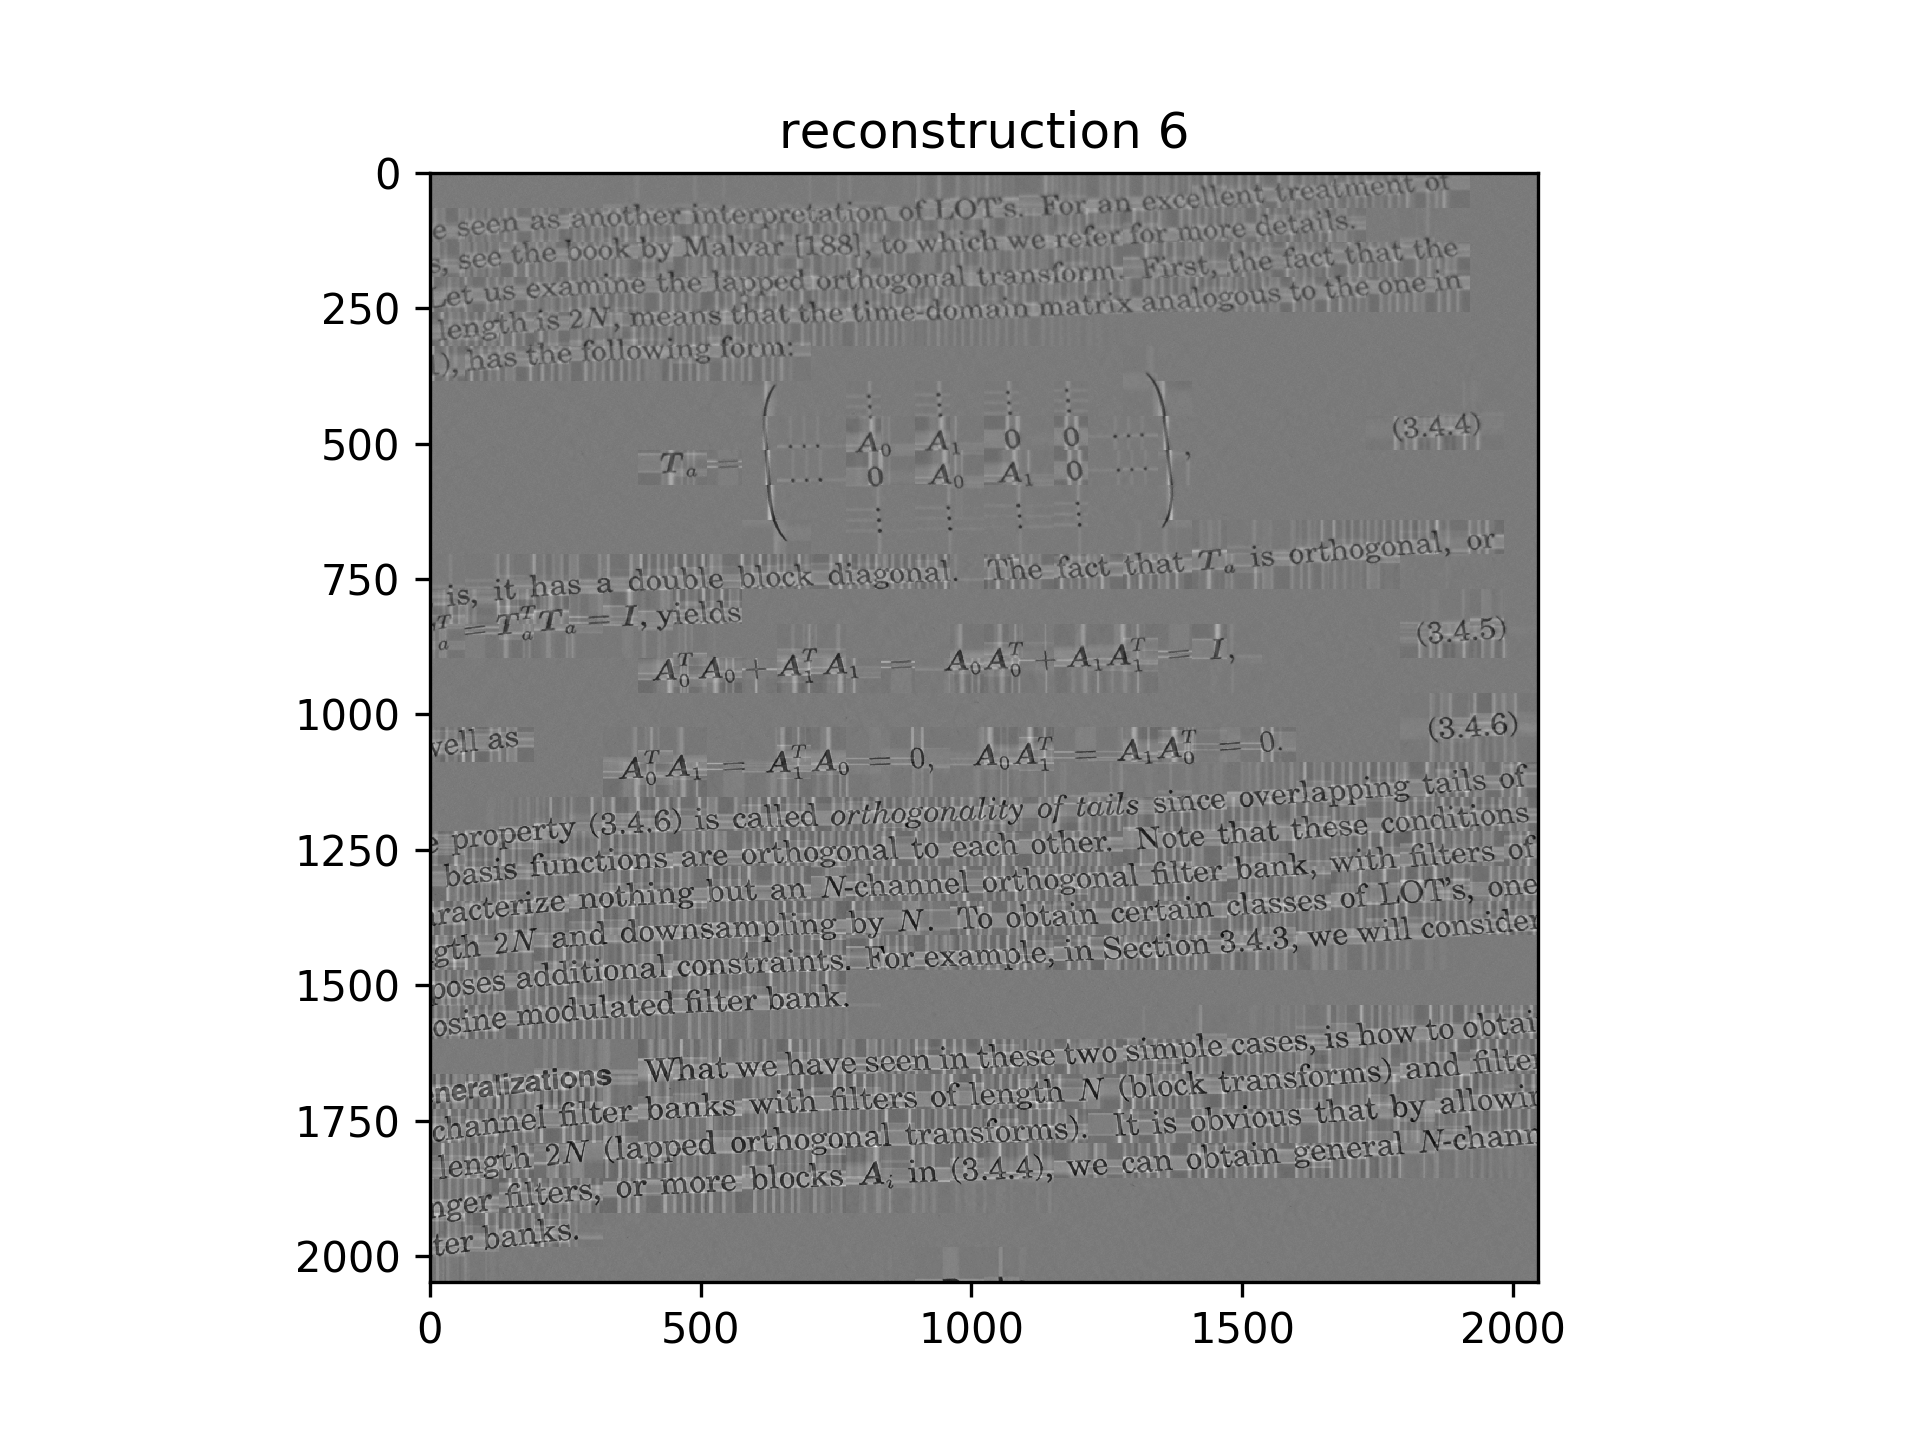
\includegraphics[width=8cm]{images/book_r_h_6.png}
\caption{Libro reconstruido tomando los coeficientes más altos de la DWT de nivel 6}
\end{figure}






\section{Análisis}

En los casos de compresión, vemos que esta compresión hecha sin mucha sofisticación es \emph{con pedidas}, pero de todas maneras puede ser útil para aplicaciones donde alta resolución no sea un requisito, como por ejemplo detección de objetos \cite{pedestrian}, donde puede bajarse la resolución para ahorrar tiempo en los cálculos. Lo más interesante es notar que usando solo 1/4 de la información original, es posible reconstruir una imagen con pérdidas casi imperceptibles. Efectivamente hay pérdidas, se pueden ve a continuación, donde definimos el error en la imagen como otra imagen dada por:


\begin{equation}
  \text{error} = \hat{\pmb{x}}-\pmb{x}
\end{equation}

Donde $\hat{\pmb{x}}$ es la matriz reconstruida.



\begin{figure}[H]
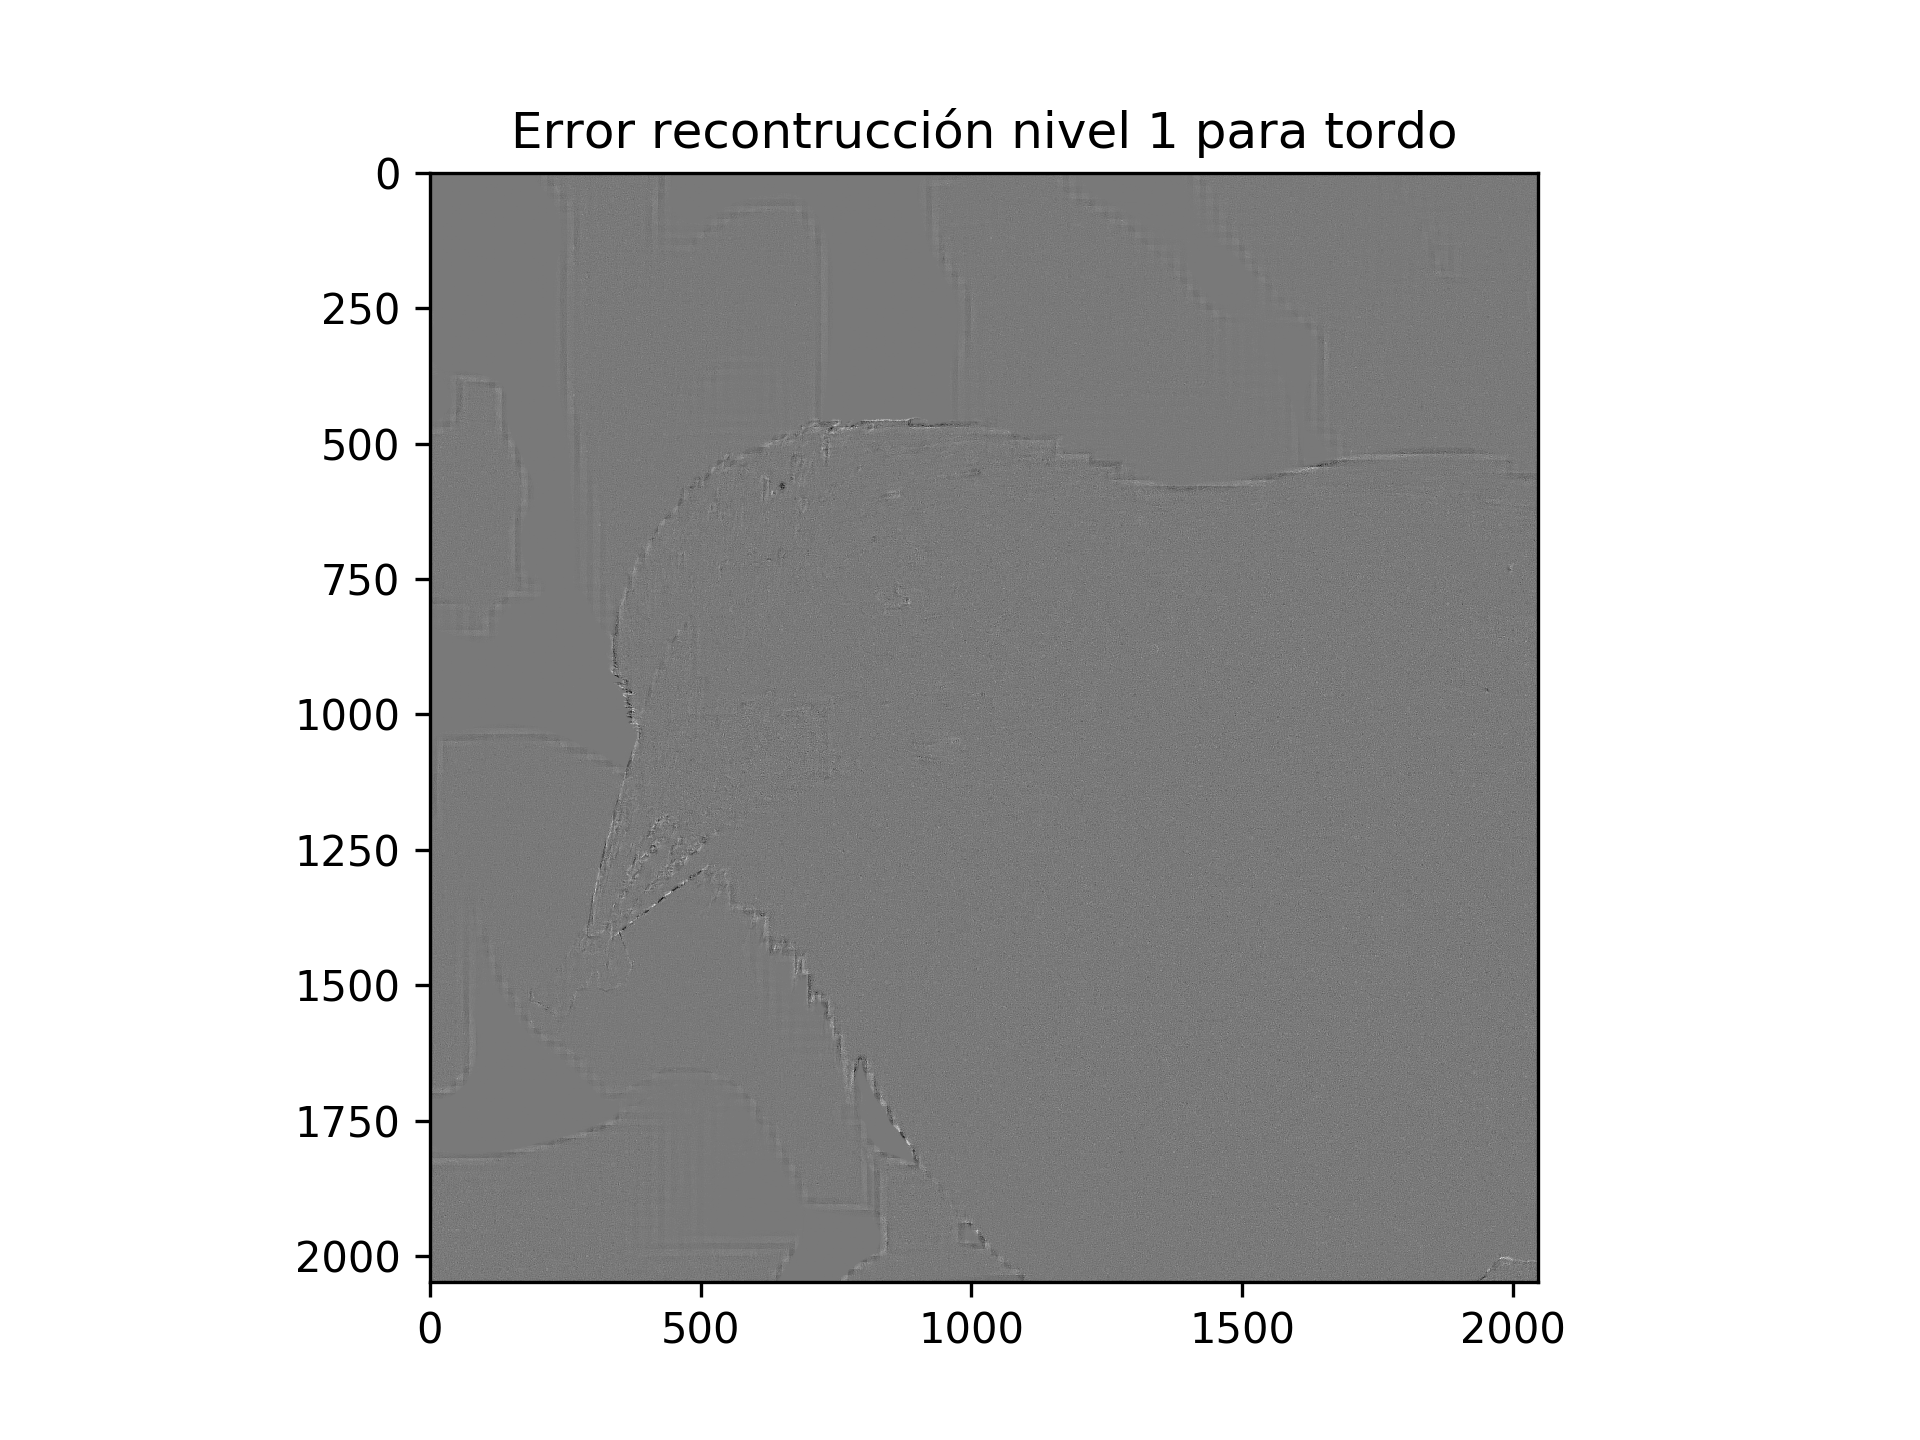
\includegraphics[width=8cm]{images/error_tordo_r_1.png}
\caption{Error para la reconstrucción de los coeficientes bajos para la DWT de nivel 1 para el tordo}
\end{figure}


Podemos notar que el error es más grande (píxeles más oscuros) en los bordes de los objetos (ave y hojas del árbol), lo cual es consistente con las características cualitativas de las wavelets, ya que al usar solo los coeficientes bajos, estamos perdiendo detalles de alta frecuencia que están justamente en los bordes.

Notamos que para la parte de resaltado de bordes, las altas frecuencias son las más presentes, pero también a medida que tomamos DWT de nivel cada vez más alto, la parte que llamamos ``alta frecuencia'' contiene cada vez más información ya que estos coeficientes no son estrictamente los coeficientes $\Phi$ discutidos en secciones anteriores, sino que es más bien un corte arbitrario hecho por simplicidad, la parte de ``bajas frecuencias'' corresponde a los primeros $N/(2^\text{nivel})$ valores tanto para las filas como para las columnas, mientras que las ``altas frecuencias'' son son los últimos $N(2^\text{nivel}-1)/2^\text{nivel}$ también en filas y columnas, pese a esto muestra bastante bien el comportamiento de las wavelets\footnote{Recordemos que en todo esto, estamos hablando de vectores que son matrices de $N\text{x}N$}.

\section{Limitaciones}

La primera limitación de esta implementación salta a la vista en el título de este trabajo, solo sirve para el caso de la wavelet Haar. Esto es importante, ya que como fue comentado en secciones anteriores, hay infinitas wavelets y las conocidas si bien evidentemente no son todas, son muchas más que una.

Otra limitación tiene que ver con el nivel al que podemos llegar de wavelets, vemos que depende del tamaño de nuestra matriz, ya que hay $J = \log_2 N$ niveles de descomposición. El problema es que es necesario un vector con, evidentemente, $N=2^J$, es decir, $N$ tiene que ser una potencia de $2$. El mayor problema de esto es que a medida que aumentamos el tamaño de nuestro vector $\pmb{x}$, un ``error'' en el tamaño necesitado de una unidad, implica grandes pérdidas en información para llevar a cabo el análisis. A modo de ejemplo, imaginémonos un vector de tamaño $N=2^J-1$, esto significa que este vector no puede utilizarse, al menos no con esta implementación, y vamos a tener que tomar la potencia de 2 más cercana $N'=2^{J-1}$, lo que implica una pérdida del orden de $2^{J-1}$ lo cual para $J$ grandes, implica pérdidas de información importantes. Una posible solución es analizar de a trozos, pero no es muy eficiente y reduce el número de niveles de wavelets disponibles para explorar.

\section{Conclusiones}

En este trabajo exploramos los fundamentos matemáticos que motivan la creación de las wavelets, así como una implementación en Python del caso Haar en dos dimensiones.Notamos también la diferencia en contenido frecuencial entre distintas escalas y cómo puede ser aprovechado tanto en el problema de compresión como en el problema de detección de bordes y objetos. Lo anterior nos permite ver que las wavelets, en su esencia, no son muy distintas a cualquier otra base que podamos encontrar, pero sí el hecho de poder diseñarlas en función de los requerimientos deseados \cite{wavelettour} y el que puedan ser implementadas como bancos de filtros, hacen que se transforman inmediatamente en herramientas muy útiles en el análisis de señales. También la introducción del análisis multiresolución hace que sean muy llamativas en distintas áreas. Además se han hecho estudios sobre la escalabilidad de los algoritmos para computar wavelets para permitir su aplicación en grandes problemas \cite{esc}.
En resumen, las wavelets, es un área que vale la pena explorar, sobretodo algoritmos que permitan su rápida ejecución en arquitecturas de computación paralela \cite{paralela}, cada vez más populares y utilizadas.



\section{Código fuente}
Todo el código utilizado para la realización de este trabajo puede encontrarse en este repositorio:
\textcolor{blue}{\url{https://github.com/tomasrojasc/Implementation-of-the-Haar-2-D-DWT}}
\newline
\newline
\bibliography{bibliography}



\end{document}
